\باب{یک سمت  رو مشین}\شناخت{باب_یک_سمتی_رو_مشین}
\اصطلاح{یک سمت  رو مشین}\فرہنگ{یک سمت  رو!مشین}  یک سمت  رو\حاشیہب{dc, direct current} برقی طاقت پیدا کرتی ہیں یا یک سمت  رو برقی طاقت سے چلتی ہیں۔یک سمت  رو موٹروں کی اہمیت بتدریج کم ہو رہی ہے اور ان کی جگہ امالی موٹر لے رہے ہیں جن کی رفتار  \اصطلاح{قوی برقیات}\فرہنگ{قوی برقیات}\حاشیہب{power electronics} سے قابو کی جاتی ہے۔موجودہ دور میں گاڑیوں کے یک سمت  جنریٹر بھی دراصل سادہ بدلتا رو جنریٹر ہوتے ہیں جن کے اندر نسب \اصطلاح{ڈایوڈ}\حاشیہب{diode}  بدلتا محرک برقی دباو کو یک سمت  محرک برقی دباو میں تبدیل کرتے ہیں۔

اس باب میں دو قطب کے یک سمت  مشینوں کا مطالعہ کیا جائے گا۔میکانی سمت کار  والے یک سمت  مشینوں میں میدانی لچھا ساکن  جبکہ قوی لچھا گھومتا ہے۔

\حصہ{میکانی سمت کار کی بنیادی کارکردگی}
جنریٹر بنیادی طور پر بدلتا برقی دباو پیدا کرتا ہے۔ یک سمت  جنریٹر کے اندر نسب  میکانی \اصطلاح{سمت کار}\فرہنگ{سمت کار}\فرہنگ{commutator}\حاشیہب{commutator} میکانی طریقہ سے بدلتا دباو کو یک سمت  دباو میں تبدیل کر کے برقی سروں پر فراہم کرتا ہے۔

میکانی سمت کار کو شکل \حوالہ{شکل_یکسمتی_میکانی_سمتکار}  میں دکھایا گیا ہے جہاں جنریٹر کے قوی  لچھے کو ایک چکر کا دکھایا گیا ہے اگرچہ حقیقت میں لچھا زیادہ چکر کا ہو گا۔قوی لچھے کے برقی سروں کو د اور ڈ سے ظاہر کیا گیا ہے جو سمت کار کے د اور ڈ حصوں کے ساتھ جڑے ہیں۔قوی لچھا اور سمت کار ایک ہی دھرے پر نسب ہوتے ہیں لہٰذا دونوں ایک ساتھ حرکت کرتے ہیں۔تصور کریں  (میکانی سمت کار سے لچھے کی طرف دیکھتے ہوئے)   مقناطیسی میدان میں دونوں  گھڑی وار گھوم رہے ہیں۔مقناطیسی میدان  افقی سطح میں \عددیء{N} سے \عددیء{S} رخ ہو گا جسے نوکدار لکیروں سے دکھایا گیا ہے۔ سمت کار کے ساتھ ساکن  کاربن بش، اسپرنگ کی مدد سے دبا کر رکھے جاتے ہیں۔ان کاربن بشوں سے برقی دباو کو جنریٹر کے باہر   منتقل کیا جاتا ہے۔ بشوں کو مثبت علامت \عددیء{+}  اور منفی علامت  \عددیء{-} سے ظاہر کیا گیا ہے۔
\begin{figure}
\centering
%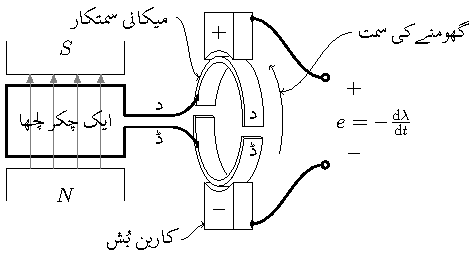
\includegraphics{figDCcommutatorA}
\begin{tikzpicture}[xscale=0.4,yscale=1]
\pgfmathsetmacro{\cRi}{1}  %commutator inner radius
\pgfmathsetmacro{\cRo}{\cRi+0.1}  %commutator inner radius
\pgfmathsetmacro{\cW}{0.8}   %commutator width
\pgfmathsetmacro{\cT}{\cRo-\cRi}    %commutator thickness
\pgfmathsetmacro{\tilt}{-10}
\pgfmathsetmacro{\gap}{5}     %gap between commutator pieces
\pgfmathsetmacro{\bush}{30}   %bush as half angle
\pgfmathsetmacro{\bR}{\cRo+0.1}   %bush radius
\pgfmathsetmacro{\coilW}{0.5}
\pgfmathsetmacro{\coilL}{5}
\pgfmathsetmacro{\coilLdel}{4}
\pgfmathsetmacro{\coilWdel}{0.1}
%upper commutator
\path[fill=white] (\tilt+\gap:\cRi)coordinate(fillA) arc (\tilt+\gap:180+\tilt-\gap:\cRi)coordinate(fillB) --++(180+\tilt-\gap:\cT)coordinate(fillC) arc (180+\tilt-\gap:90:\cRo)coordinate(fillD)--++(\cW,0)coordinate(fillE) arc (90:\tilt+\gap:\cRo)coordinate(fillF)--++(-\cW,0)coordinate(fillG) --cycle;
\path (\tilt+\gap:\cRi)coordinate(aA) arc (\tilt+\gap:180+\tilt-\gap:\cRi)coordinate(aB) --++(180+\tilt-\gap:\cT)coordinate(aC) arc (180+\tilt-\gap:\tilt+\gap:\cRo)coordinate(aD)--cycle;
\path(aD)--++(\cW,0)coordinate(bA) arc (\tilt+\gap:90:\cRo)coordinate(bB)--++(-\cW,0)coordinate(bC);
\path(aB)--++(\cW,0)coordinate(cA) arc (180+\tilt-\gap:\tilt+\gap:\cRi)coordinate(cB);
%
\draw (90+\bush:\bR)--++(\cW,0); %upper bush lower back horizontal edge
\draw(aB)--++(\cW,0) arc (180+\tilt-\gap:\tilt+\gap:\cRi);
\path[fill=white] (\tilt+\gap:\cRi) arc (\tilt+\gap:180+\tilt-\gap:\cRi) --++(180+\tilt-\gap:\cT) arc (180+\tilt-\gap:90:\cRo)--++(\cW,0) arc (90:\tilt+\gap:\cRo)--++(-\cW,0) --cycle;
\draw (\tilt+\gap:\cRi) arc (\tilt+\gap:180+\tilt-\gap:\cRi) --++(180+\tilt-\gap:\cT) arc (180+\tilt-\gap:\tilt+\gap:\cRo)--cycle;
\draw(aD)--++(\cW,0) arc (\tilt+\gap:90:\cRo)--++(-\cW,0);

%upper bush
\path (90+\bush:\bR)coordinate(bbA) arc (90+\bush:90-\bush:\bR)coordinate(bbB) --++(\cW,0)coordinate(bbC)--++(0,\cW)coordinate(bbD)--++(-\cW,0)coordinate(bbE)--++(0,-\cW);
\path(bbA)--++(0,\cW)coordinate(bbF)--(bbE);
\path[fill=white] (90+\bush:\bR) arc (90+\bush:90-\bush:\bR) --(bbE)--(bbF)--cycle;
\path[fill=white](bbB)--(bbC)--(bbD)--(bbE)--cycle;
%
\draw (90+\bush:\bR) arc (90+\bush:90-\bush:\bR) --++(\cW,0)--++(0,\cW)--++(-\cW,0)--++(0,-\cW);
\draw(bbA)--++(0,\cW)--(bbE);
%
%lower commutator
\path (180+\tilt+\gap:\cRi)coordinate(aA) arc (180+\tilt+\gap:180+180+\tilt-\gap:\cRi)coordinate(aB)--++(180+180+\tilt-\gap:\cT)coordinate(aC) arc (180+180+\tilt-\gap:180+\tilt+\gap:\cRo)coordinate(aD)--cycle;
\path(aB)--++(\cW,0)coordinate(aaA)--++(\tilt-\gap:\cT)coordinate(aaB)--++(-\cW,0);
\path(aD)--++(\cW,0)coordinate(aaC)--++(\tilt-\gap:\cT)coordinate(aaD)--++(-\cW,0);
\path (aaD) arc (180+\tilt+\gap:180+180+\tilt-\gap:\cRi);
\path(aaB) arc (180+180+\tilt-\gap:270:\cRo)coordinate(aaE)--++(-\cW,0)coordinate(aaF);
%lower bush
\path(270-\bush:\bR)coordinate(bbbA) arc (270-\bush:270+\bush:\bR)coordinate(bbbB)--++(\cW,0)coordinate(bbbC)--++(0,-\cW)coordinate(bbbD)--++(-\cW,0)coordinate(bbbE)--++(0,\cW);
\path(270-\bush:\bR) --++(0,-\cW)--(bbbE);
\path (bbbA)--++(\cW,0)coordinate(bbbG) arc (270-\bush:270+\bush:\bR);
\path (bbbA)++(0,-\cW)coordinate(bbbF);
%========
\draw(bbbA)--++(\cW,0)coordinate(bbbG) arc (270-\bush:270+\bush:\bR);
\draw (aaD) arc (180+\tilt+\gap:180+180+\tilt-\gap:\cRi);
\path[fill=white](aA) arc (180+\tilt+\gap:180+180+\tilt-\gap:\cRi) --(aaA)--(aaB)  arc (180+180+\tilt-\gap:270:\cRo)--++(-\cW,0) arc (270:180+\tilt-\gap:\cRo)--cycle;
\draw (180+\tilt+\gap:\cRi) arc (180+\tilt+\gap:180+180+\tilt-\gap:\cRi)--++(180+180+\tilt-\gap:\cT) arc (180+180+\tilt-\gap:180+\tilt+\gap:\cRo)--cycle;
\draw(aB)--++(\cW,0)--++(\tilt-\gap:\cT)--++(-\cW,0);
\draw(aD)--++(\cW,0)--++(\tilt-\gap:\cT)--++(-\cW,0);
\draw(aaB) arc (180+180+\tilt-\gap:270:\cRo)--++(-\cW,0);
%lower bush
\path[fill=white](bbbA) arc (270-\bush:270+\bush:\bR)--++(\cW,0)--++(0,-\cW)--++(-\cW,0)--(bbbF)--cycle;
\draw(270-\bush:\bR)coordinate(bbbA) arc (270-\bush:270+\bush:\bR)coordinate(bbbB)--++(\cW,0)coordinate(bbbC)--++(0,-\cW)coordinate(bbbD)--++(-\cW,0)coordinate(bbbE)--++(0,\cW);
\draw(270-\bush:\bR) --++(0,-\cW)--(bbbE);
%grid
%\draw[gray] (-10,-5) grid (4,3);
%coil
\draw[thick] (-\coilLdel,-\coilWdel)coordinate(coilS)--++(0,-\coilW)--++(-\coilL,0)--++(0,2*\coilW+2*\coilWdel)--++(\coilL,0)--++(0,-\coilW)coordinate(coilE);
\draw[thick](coilS)--++(\coilLdel/2,0) to [out=0,in=150] (-0.9,-0.4)coordinate (coilSend) ;
\draw[thick](coilE)--++(\coilLdel/2,0) to [out=0,in=210] (-0.9,0.4)coordinate (coilEend);
\draw[fill] (coilSend) circle (1.5pt);
\draw[fill] (coilEend) circle (1.5pt);
%magnet
\draw (coilS)++(0,-2.5*\coilW)--++(0,1.5*\coilW-0.2)--++(-\coilL,0)--++(0,-1.5*\coilW+0.2);
\draw (coilE)++(0,2.5*\coilW)--++(0,-1.5*\coilW+0.2)--++(-\coilL,0)--++(0,1.5*\coilW-0.2);
\draw node at (-6.5,-1.25){$N$};
\draw node at (-6.5,1.25){$S$};
\foreach \x in {-8,-7,-6,-5}{
\draw[gray,-latex] (\x,-\coilWdel-\coilW-0.2)--++(0,2*\coilW+2*\coilWdel+0.4);}
%bush connections
\draw[thick] (bbD)++(0,-0.1) to [out=0,in=180] ++(3,-1) to [short,-o]++(0.1,0)coordinate(outputA);
\draw [fill] (bbD)++(0,-0.1) circle (1.5pt);
\draw[thick] (bbbD)++(0,0.1) to [out=0,in=180] ++(3,1)to [short,-o]++(0.1,0)coordinate(outputB);
\draw [fill] (bbbD)++(0,0.1) circle (1.5pt);
\draw node[right] at ($(outputA)!0.5!(outputB)$){$\begin{aligned}  &+\\ &e\\ &-  \end{aligned}$};
%direction of rotation
\draw[->] (2*\cW,0)++(-30:\cRo) arc (-30:60:\cRo);
\draw[<-] (2.6,0.5) to [out=0,in=180] ++(3,1)node[right]{\small{\RL{گھومنے کا رخ}}};
%text
\draw (\tilt+\gap:\cRo)++(\cW/2,0.2)node{د};
\draw (\tilt-\gap:\cRo)++(\cW/2,-0.2)node{ڈ};
\draw (90:\cRo+\cW/2)node{$+$};
\draw (270:\cRo+\cW/2)node{$-$};
\draw[<-] (-0.6,-1.75) to [out=180,in=0] ++(-1,-0.25)node[left]{\RL{کاربن بش}};
\draw[<-] (-0.8,0.75) to [out=180,in=0] ++(-1,1)node[left]{\RL{میکانی سمتکار}};
\draw node at (-2.5,0.25){د};
\draw node at (-2.5,-0.27){ڈ};
\draw node at (-6.5,0){\small{\RL{ایک چکر لچھا}}};
\end{tikzpicture}%
\caption{میکانی سمت کار۔}
\label{شکل_یکسمتی_میکانی_سمتکار}
\end{figure}

دکھائے گئے لمحہ پر لچھے میں پیدا برقی دباو \عددیء{e} کی وجہ سے لچھے کا  سر د مثبت اور  ڈ منفی ہے۔یوں سمت کار کا حصہ د مثبت اور حصہ ڈ منفی ہوں گے لہٰذا کاربن کا \عددیء{+} علامت والا بش مثبت اور \عددیء{-} علامت والا بش منفی ہو گا۔یوں بیرونی  بالائی تار مثبت اور نچلی تار  منفی ہوں گے۔ 
\begin{figure}
\centering
%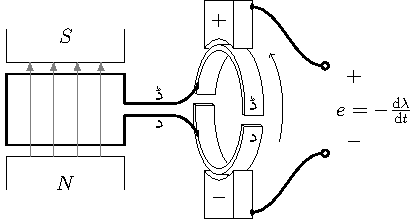
\includegraphics{figDCcommutatorB}
\begin{tikzpicture}[xscale=0.4,yscale=1]
%grid
%\draw[gray,thick] (-2*\sRo,-2*\sRo) grid (2*\sRo,3*\sRo);
%\draw[gray,thin,xstep=0.1,ystep=0.1] (-2*\sRo,-2*\sRo) grid (2*\sRo,3*\sRo);
\pgfmathsetmacro{\cRi}{1}  %commutator inner radius
\pgfmathsetmacro{\cRo}{\cRi+0.1}  %commutator inner radius
\pgfmathsetmacro{\cW}{0.8}   %commutator width
\pgfmathsetmacro{\cT}{\cRo-\cRi}    %commutator thickness
\pgfmathsetmacro{\tilt}{-10}
\pgfmathsetmacro{\gap}{5}     %gap between commutator pieces
\pgfmathsetmacro{\bush}{30}   %bush as half angle
\pgfmathsetmacro{\bR}{\cRo+0.1}   %bush radius
\pgfmathsetmacro{\coilW}{0.5}
\pgfmathsetmacro{\coilL}{5}
\pgfmathsetmacro{\coilLdel}{4}
\pgfmathsetmacro{\coilWdel}{0.1}

%upper commutator
\path[fill=white] (\tilt+\gap:\cRi)coordinate(fillA) arc (\tilt+\gap:180+\tilt-\gap:\cRi)coordinate(fillB) --++(180+\tilt-\gap:\cT)coordinate(fillC) arc (180+\tilt-\gap:90:\cRo)coordinate(fillD)--++(\cW,0)coordinate(fillE) arc (90:\tilt+\gap:\cRo)coordinate(fillF)--++(-\cW,0)coordinate(fillG) --cycle;
\path (\tilt+\gap:\cRi)coordinate(aA) arc (\tilt+\gap:180+\tilt-\gap:\cRi)coordinate(aB) --++(180+\tilt-\gap:\cT)coordinate(aC) arc (180+\tilt-\gap:\tilt+\gap:\cRo)coordinate(aD)--cycle;
\path(aD)--++(\cW,0)coordinate(bA) arc (\tilt+\gap:90:\cRo)coordinate(bB)--++(-\cW,0)coordinate(bC);
\path(aB)--++(\cW,0)coordinate(cA) arc (180+\tilt-\gap:\tilt+\gap:\cRi)coordinate(cB);
%
\draw (90+\bush:\bR)--++(\cW,0); %upper bush lower back horizontal edge
\draw(aB)--++(\cW,0) arc (180+\tilt-\gap:\tilt+\gap:\cRi);
\path[fill=white] (\tilt+\gap:\cRi) arc (\tilt+\gap:180+\tilt-\gap:\cRi) --++(180+\tilt-\gap:\cT) arc (180+\tilt-\gap:90:\cRo)--++(\cW,0) arc (90:\tilt+\gap:\cRo)--++(-\cW,0) --cycle;
\draw (\tilt+\gap:\cRi) arc (\tilt+\gap:180+\tilt-\gap:\cRi) --++(180+\tilt-\gap:\cT) arc (180+\tilt-\gap:\tilt+\gap:\cRo)--cycle;
\draw(aD)--++(\cW,0) arc (\tilt+\gap:90:\cRo)--++(-\cW,0);

%upper bush
\path (90+\bush:\bR)coordinate(bbA) arc (90+\bush:90-\bush:\bR)coordinate(bbB) --++(\cW,0)coordinate(bbC)--++(0,\cW)coordinate(bbD)--++(-\cW,0)coordinate(bbE)--++(0,-\cW);
\path(bbA)--++(0,\cW)coordinate(bbF)--(bbE);
\path[fill=white] (90+\bush:\bR) arc (90+\bush:90-\bush:\bR) --(bbE)--(bbF)--cycle;
\path[fill=white](bbB)--(bbC)--(bbD)--(bbE)--cycle;
%
\draw (90+\bush:\bR) arc (90+\bush:90-\bush:\bR) --++(\cW,0)--++(0,\cW)--++(-\cW,0)--++(0,-\cW);
\draw(bbA)--++(0,\cW)--(bbE);
%
%lower commutator
\path (180+\tilt+\gap:\cRi)coordinate(aA) arc (180+\tilt+\gap:180+180+\tilt-\gap:\cRi)coordinate(aB)--++(180+180+\tilt-\gap:\cT)coordinate(aC) arc (180+180+\tilt-\gap:180+\tilt+\gap:\cRo)coordinate(aD)--cycle;
\path(aB)--++(\cW,0)coordinate(aaA)--++(\tilt-\gap:\cT)coordinate(aaB)--++(-\cW,0);
\path(aD)--++(\cW,0)coordinate(aaC)--++(\tilt-\gap:\cT)coordinate(aaD)--++(-\cW,0);
\path (aaD) arc (180+\tilt+\gap:180+180+\tilt-\gap:\cRi);
\path(aaB) arc (180+180+\tilt-\gap:270:\cRo)coordinate(aaE)--++(-\cW,0)coordinate(aaF);
%lower bush
\path(270-\bush:\bR)coordinate(bbbA) arc (270-\bush:270+\bush:\bR)coordinate(bbbB)--++(\cW,0)coordinate(bbbC)--++(0,-\cW)coordinate(bbbD)--++(-\cW,0)coordinate(bbbE)--++(0,\cW);
\path(270-\bush:\bR) --++(0,-\cW)--(bbbE);
\path (bbbA)--++(\cW,0)coordinate(bbbG) arc (270-\bush:270+\bush:\bR);
\path (bbbA)++(0,-\cW)coordinate(bbbF);
%========
\draw(bbbA)--++(\cW,0)coordinate(bbbG) arc (270-\bush:270+\bush:\bR);
\draw (aaD) arc (180+\tilt+\gap:180+180+\tilt-\gap:\cRi);
\path[fill=white](aA) arc (180+\tilt+\gap:180+180+\tilt-\gap:\cRi) --(aaA)--(aaB)  arc (180+180+\tilt-\gap:270:\cRo)--++(-\cW,0) arc (270:180+\tilt-\gap:\cRo)--cycle;
\draw (180+\tilt+\gap:\cRi) arc (180+\tilt+\gap:180+180+\tilt-\gap:\cRi)--++(180+180+\tilt-\gap:\cT) arc (180+180+\tilt-\gap:180+\tilt+\gap:\cRo)--cycle;
\draw(aB)--++(\cW,0)--++(\tilt-\gap:\cT)--++(-\cW,0);
\draw(aD)--++(\cW,0)--++(\tilt-\gap:\cT)--++(-\cW,0);
\draw(aaB) arc (180+180+\tilt-\gap:270:\cRo)--++(-\cW,0);
%lower bush
\path[fill=white](bbbA) arc (270-\bush:270+\bush:\bR)--++(\cW,0)--++(0,-\cW)--++(-\cW,0)--(bbbF)--cycle;
\draw(270-\bush:\bR)coordinate(bbbA) arc (270-\bush:270+\bush:\bR)coordinate(bbbB)--++(\cW,0)coordinate(bbbC)--++(0,-\cW)coordinate(bbbD)--++(-\cW,0)coordinate(bbbE)--++(0,\cW);
\draw(270-\bush:\bR) --++(0,-\cW)--(bbbE);
%grid
%\draw[gray] (-10,-5) grid (4,3);
%coil
\draw[thick] (-\coilLdel,-\coilWdel)coordinate(coilS)--++(0,-\coilW)--++(-\coilL,0)--++(0,2*\coilW+2*\coilWdel)--++(\coilL,0)--++(0,-\coilW)coordinate(coilE);
\draw[thick](coilS)--++(\coilLdel/2,0) to [out=0,in=150] (-0.9,-0.4)coordinate (coilSend) ;
\draw[thick](coilE)--++(\coilLdel/2,0) to [out=0,in=210] (-0.9,0.4)coordinate (coilEend);
\draw[fill] (coilSend) circle (1.5pt);
\draw[fill] (coilEend) circle (1.5pt);
%magnet
\draw (coilS)++(0,-2.5*\coilW)--++(0,1.5*\coilW-0.2)--++(-\coilL,0)--++(0,-1.5*\coilW+0.2);
\draw (coilE)++(0,2.5*\coilW)--++(0,-1.5*\coilW+0.2)--++(-\coilL,0)--++(0,1.5*\coilW-0.2);
\draw node at (-6.5,-1.25){$N$};
\draw node at (-6.5,1.25){$S$};
\foreach \x in {-8,-7,-6,-5}{
\draw[gray,-latex] (\x,-\coilWdel-\coilW-0.2)--++(0,2*\coilW+2*\coilWdel+0.4);}
%bush connections
\draw[thick] (bbD)++(0,-0.1) to [out=0,in=180] ++(3,-1) to [short,-o]++(0.1,0)coordinate(outputA);
\draw [fill] (bbD)++(0,-0.1) circle (1.5pt);
\draw[thick] (bbbD)++(0,0.1) to [out=0,in=180] ++(3,1)to [short,-o]++(0.1,0)coordinate(outputB);
\draw [fill] (bbbD)++(0,0.1) circle (1.5pt);
\draw node[right] at ($(outputA)!0.5!(outputB)$){$\begin{aligned}  &+\\ &e\\ &-  \end{aligned}$};
%direction of rotation
\draw[->] (2*\cW,0)++(-30:\cRo) arc (-30:60:\cRo);
%text
\draw (\tilt+\gap:\cRo)++(\cW/2,0.2)node{ڈ};
\draw (\tilt-\gap:\cRo)++(\cW/2,-0.2)node{د};
\draw (90:\cRo+\cW/2)node{$+$};
\draw (270:\cRo+\cW/2)node{$-$};
\draw node at (-2.5,0.27){ڈ};
\draw node at (-2.5,-0.25){د};
\end{tikzpicture}
\caption{آدھے چکر کے بعد بھی بالائی  بُش مثبت ہی ہے۔}
\label{شکل_یکسمتی_میکانی_سمتکار_آدھے_چکر_بعد}
\end{figure}
آدھا چکر بعد، جیسا شکل \حوالہ{شکل_یکسمتی_میکانی_سمتکار_آدھے_چکر_بعد}  میں دکھایا گیا ہے،  خلائی درز میں لچھا کے د اور ڈ اطراف آپس میں جگہیں تبدیل کر چکے ہوں گے ۔لچھا کے د اور ڈ اطراف اب بھی سمت کار کے د اور ڈ حصوں کے ساتھ جڑے ہیں۔ لچھے پر برقی دباو الٹ ہے اور اس کا سر د منفی اور ڈ مثبت ہیں۔یہاں سمت کار کی کارکردگی پر نظر رکھیں۔ اب بھی کاربن کا \عددیء{+}  علامت والا بش  مثبت اور \عددیء{-} علامت والا بش منفی ہے۔ یوں جنریٹر کے بیرونی برقی سروں پر اب بھی بالائی سر مثبت اور نچلا سر منفی ہے۔سمت کار کے دانتوں کے مابین برقی دباو ہوتا ہے لہٰذا ان کو غیر موصل  کی مدد سے ایک دوسرے اور دھرے سے دور رکھا جاتا ہے۔

گھومتے وقت ایک ایسا لمحہ آتا ہے جب سمت کار کے  دانتوں کو کاربن بش  قصر دور کرتے ہیں۔ کاربن بش  محیط پر اس طرح رکھے جاتے ہیں کہ جس لمحہ لچھے میں برقی دباو مثبت سے منفی یا منفی سے مثبت ہونا چاہے اسی لمحہ کاربن کے بش لچھے کو قصر دور کرتے ہوں۔چونکہ اس لمحہ  لچھے پر محرک  دباو صفر ہوتا ہے لہٰذا اسے قصر دور کرنے سے کوئی نقصان نہیں ہوتا ہے۔یوں حاصل برقی دباو شکل \حوالہ{شکل_یکسمتی_دو_دندوں_کا_سمتکار}  میں دکھایا گیا ہے۔
\begin{figure}
\centering
%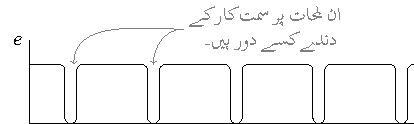
\includegraphics{figDCcommutatorVoltage}
\begin{tikzpicture}
%grid
%\draw[gray] (-1,0) grid (7,2);
%
\pgfmathsetmacro{\x}{1}
\pgfmathsetmacro{\y}{0.8}

\newcommand{\ripple}{to [out=0,in=90] ++(0.1,-0.1)--++(0,-\y) to [out=-90,in=180]++(0.1,-0.1) to [out=0,in=-90]++(0.1,0.1) --++(0,\y) to [out=90,in=180]++(0.1,0.1)}
%ripple
\draw (0,1)--++(\x/2,0)  \ripple --++(\x,0)  \ripple--++(\x,0)  \ripple--++(\x,0)  \ripple--++(\x,0)  \ripple;  
%axis
\draw (0,0)--(0,1.4) node[left]{$e$};
\draw (0,0)--(6.5,0);
%
\draw [] (2.1,1) to [out=90, in=180] ++(0.5,0.6)node[right,align=right](text){\small \RL{ان لمحات پر سمت کار کے}\\  \small \RL{ دندے قصرے دور ہیں۔}};
\draw[](0.75,1) to [out=90,in=180] (text);
\end{tikzpicture}
\caption{دو دندی سمت کار سے حاصل یک سمت  برقی دباو۔}
\label{شکل_یکسمتی_دو_دندوں_کا_سمتکار}
\end{figure}


یہاں دو دندی سمت کار اور دو مقناطیسی قطب کے درمیان گھومتا ہوا ایک قوی لچھا دکھایا گیا ہے۔حقیقت میں جنریٹر کے متعدد قطبین ہوں گے اور فی قطب  سمت کار کے کئی دندے ہوں گے۔چھوٹی مشینوں میں مقناطیس ہی مقناطیسی میدان  فراہم کرتا ہے جبکہ بڑی مشینوں میں مقناطیسی میدان ساکن میدانی لچھے فراہم کرتے ہیں۔ دونوں اقسام کی مشینوں  کے لچھے تقسیم شدہ ہوتے ہیں۔

اب ہم زیادہ دندوں کے ایک سمت کار کو دیکھتے ہیں۔

\جزوحصہ{میکانی سمت کار کی تفصیل}
پچھلے حصہ میں سمت کار کی بنیادی کارکردگی پر غور کیا گیا۔ اس حصہ میں اس پر تفصیلی بات کی جائے گی۔ شکل \حوالہ{شکل_یکسمتی_سمتکار_بش_کسر_دور_نہیں_کر_رہا} میں امالی مشین دکھائی گئی ہے۔اس شکل میں اندر کو سمت کار ہے جس کے دندوں کو گنتی لگائی گئی ہے۔سمت کار کی اندر جانب دو عدد  کاربن بش ہیں جن سے   بیرون  برقی رو \عددی{i} حاصل کی جاتی ہے۔شگافوں کو بھی گنتی لگائی گئی  ہے۔جنریٹر کے دو قطب اور آٹھ شگاف ہیں۔اس طرح اگر ایک شگاف ایک قطب کے سامنے ہو تو تین شگاف چھوڑ کر موجود شگاف دوسرے قطب کے سامنے ہو گا۔ہم کہتے ہیں کہ ایسے دو شگاف "ایک قطب فاصلہ" پر ہیں۔یوں شگاف \عددی{1} اور \عددی{5} ایک دوسرے سے ایک قطب کے فاصلے پر ہیں جبکہ    شگاف \عددی{2} اور \عددی{6} ایک دوسرے سے ایک قطب کے فاصلے پر ہیں۔

جیسا شکل \حوالہ{شکل_یکسمتی_میکانی_سمتکار_آدھے_چکر_بعد} میں دکھایا گیا، اگر لچھے کا ایک طرف شمالی قطب کے سامنے ہو تب اس کا دوسرا طرف، ایک قطب فاصلہ پر، جنوبی قطب کے سامنے ہو گا۔لچھوں کو شگافوں میں رکھا جاتا ہے۔ یوں شکل \حوالہ{شکل_یکسمتی_سمتکار_بش_کسر_دور_نہیں_کر_رہا} میں اگر ایک لچھے کا ایک طرف شگاف \عددی{1} میں ہو تب اس کا دوسرا طرف، ایک قطب فاصلہ پر، شگاف \عددی{5} میں ہو گا۔حقیقت میں ہر شگاف میں دو لچھے رکھے جاتے ہیں۔ ایک لچھے کو شگاف میں محور کے قریب اور دوسرے کو شگاف میں محور سے دور رکھا جا سکتا ہے۔ایسا کرنے کے لئے ہمیں دو مختلف جسامت کے لچھے تیار کرنے ہوں گے۔ محور کے قریب رکھا گیا لچھا جسامت میں چھوٹا جبکہ محور سے دور لچھا بڑا ہو گا۔لچھوں کو پہلے تیار کر کے بعد میں شگافوں میں رکھا جاتا ہے۔ اس سے بہتر ترکیب موجود ہے جو حقیقت میں استعمال ہوتی ہے۔

 بہتر ترکیب میں ایک لچھے کے ایک طرف کو ایک  شگاف میں محور کے قریب اور، ایک قطب فاصلہ پر، دوسرے شگاف میں محور کے دور رکھا جاتا ہے۔دوسرے لچھے کو انہیں شگافوں میں باقی دو مقامات پر رکھا جاتا ہے۔یوں دونوں لچھوں کی جسامت ایک دوسرے جیسے ہو گی اور ان میں اتنی ڈھیل ہو گی کہ انہیں شگافوں میں با آسانی رکھا جا سکے۔

\begin{figure}
\centering
%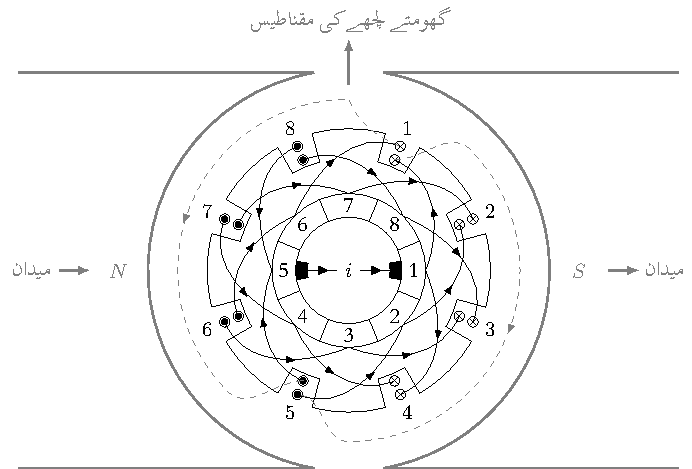
\includegraphics[scale=0.75]{figDCeightTeethCommutator}
\begin{tikzpicture}[scale=0.75]
\tikzset{->-/.style={decoration={
  markings,
  mark=at position .5 with {\arrow{latex}}},postaction={decorate}}}
\tikzset{-<-/.style={decoration={
  markings,
  mark=at position .5 with {\arrowreversed{latex}}},postaction={decorate}}}
%grid
%\draw[] (-\tR,-\tR) grid (\tR,\tR);
%
\pgfmathsetmacro{\rR}{2.4}   %stator inner radius
\pgfmathsetmacro{\tR}{\rR+0.2}
\pgfmathsetmacro{\delSlotTheta}{15}   %slot width in degrees
\pgfmathsetmacro{\delR}{0.5}     %slot radial depth
%
\commutator{8}{22.5}
\foreach \thetaA/\txt in {22.5/2,67.5/1,112.5/8,157.5/7,202.5/6,247.5/5,292.5/4,337.5/3}{\draw node at (\thetaA:\tR){$\txt$};}
%commutator teeth
\pgfmathsetmacro{\rA}{0.9}
\pgfmathsetmacro{\rB}{1.3}
\pgfmathsetmacro{\rAB}{0.5*(\rA+\rB)}
\draw (0,0) circle (\rA);
\draw (0,0) circle (\rB);
\foreach \thetaA/\txt in {22.5/2,67.5/1,112.5/8,157.5/7,202.5/6,247.5/5,292.5/4,337.5/3}{ \draw (\thetaA:\rA)--(\thetaA:\rB); \draw node at (\thetaA-67.5:\rAB){\txt};}
%bush
\draw[fill](-10:\rA) arc (-10:10:\rA)--++(10:-0.2) arc (10:-10:\rA-0.2) --cycle;
\draw[fill](170:\rA) arc (170:190:\rA)--++(190:-0.2) arc (190:170:\rA-0.2) --cycle;
\draw[] (180:\rA-0.2) to [short,i={$$}] (-0.2,0);
\draw (0.2,0)to [short,i={$$}] (0:\rA-0.2);
\draw[fill=white] node at (0,0){$i$};
%dots
\foreach \thetaA in {112.5,157.5,202.5,247.5}{
\draw (\thetaA:\rR-\delR/4) circle (2.5pt);
\draw[fill] (\thetaA:\rR-\delR/4) circle (1.5pt);
\draw (\thetaA:\rR-3*\delR/4) circle (2.5pt);
\draw[fill] (\thetaA:\rR-3*\delR/4) circle (1.5pt);  } 
%cross
\foreach \thetaA in {22.5,67.5,292.5,337.5}{
\draw (\thetaA:\rR-\delR/4) circle (2.5pt);
\draw (\thetaA:\rR-\delR/4)++(45:2.2pt)--++(-135:4.4pt);
\draw (\thetaA:\rR-\delR/4)++(-45:2.2pt)--++(135:4.4pt); 
\draw (\thetaA:\rR-3*\delR/4) circle (2.5pt);
\draw (\thetaA:\rR-3*\delR/4)++(45:2.2pt)--++(-135:4.4pt);
\draw (\thetaA:\rR-3*\delR/4)++(-45:2.2pt)--++(135:4.4pt);}
%arcs to inner side
\foreach \thetaA in {67.5}{
\draw[->-,thick] (\thetaA-67.5:\rB) to [out=\thetaA,in=\thetaA-90] (\thetaA:\rR-3*\delR/4);} %thick line 
\foreach \thetaA in {22.5,67.5,292.5,337.5}{
\draw[->-] (\thetaA-67.5:\rB) to [out=\thetaA,in=\thetaA-90] (\thetaA:\rR-3*\delR/4);    %to inner crosses
\draw[->-] (\thetaA+67.5:\rB) to [out=\thetaA,in=\thetaA+90] (\thetaA:\rR-\delR/4);}     %to outer crosses
\foreach \thetaA in {112.5,157.5,202.5,247.5}{
\draw[-<-] (\thetaA-67.5:\rB) to [out=\thetaA,in=\thetaA-90] (\thetaA:\rR-3*\delR/4);   %to inner dots
\draw[-<-] (\thetaA+67.5:\rB) to [out=\thetaA,in=\thetaA+90] (\thetaA:\rR-\delR/4);}    %to outer dots
%gray arc showing back connections
\draw[,dashed,->-] (67.5:\rR-3*\delR/4) to [out=0,in=135] (45:\rR+0.5) arc  (45:-90:\rR+0.5) to [out=180,in=-60] (-112.5:\rR-\delR/4);
\draw[,dashed,-<-] (-112.5:\rR-3*\delR/4) to [out=180,in=-45] (-135:\rR+0.5) arc  (-135:-270:\rR+0.5) to [out=0,in=100] (-292.5:\rR-\delR/4);
%external magnet
\pgfmathsetmacro{\sp}{1}
\draw[,thick] (100:\rR+\sp) arc (100:260:\rR+\sp)--++(-5,0);
\draw[,thick](100:\rR+\sp)--++(-5,0);
\draw[,thick] node at (180:\rR+1.5){$N$};
\draw[,thick] (80:\rR+\sp) arc (80:-80:\rR+\sp)--++(5,0);
\draw[,thick](80:\rR+\sp)--++(5,0);
\draw[,thick] node at (0:\rR+1.5){$S$};
%direction of mmf
\draw[,thick,-latex] (90:\rR+0.75)--++(0,0.75)node[above]{\RL{گھومتے لچھے کا مقناطیس}};
\draw[,thick,-latex]  (180:\rR+2.5)node[left]{میدان}--++(0.5,0);
\draw[,thick,-latex]  (0:\rR+2)--++(0.5,0)node[right]{میدان};
\end{tikzpicture}
\caption{کاربن بش سمتکار کے دندوں کو قصر دور نہیں کر رہا ہے۔}
\label{شکل_یکسمتی_سمتکار_بش_کسر_دور_نہیں_کر_رہا}
\end{figure}

اب شکل \حوالہ{شکل_یکسمتی_سمتکار_بش_کسر_دور_نہیں_کر_رہا} کو تفصیل سے سمجھتے ہیں۔شگافوں میں موجود لچھوں میں برقی رو کے رخ نقطہ اور صلیب سے ظاہر کئے گئے ہیں۔ نقطہ کا نشان، صفحہ سے عمودی  باہر رخ رو  کو ظاہر کرتا ہے جبکہ صلیب کا نشان اس کے مخالف رخ رو کو ظاہر کرتا ہے۔یوں پہلا \عددی{(1)} شگاف میں برقی رو   صفحہ کو عمودی اندر رخ ہے۔
\begin{figure}
\centering
%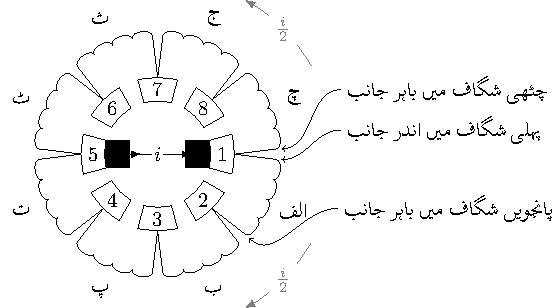
\includegraphics{figDCeightTeethCommutatorShowingCoilConnections}
\begin{tikzpicture}
\tikzset{->-/.style={decoration={
  markings,
  mark=at position .5 with {\arrow{latex}}},postaction={decorate}}}
\tikzset{-<-/.style={decoration={
  markings,
  mark=at position .5 with {\arrowreversed{latex}}},postaction={decorate}}}
%grid
%\draw[gray] (-\tR,-\tR) grid (\tR,\tR);
%
\pgfmathsetmacro{\rR}{2.4}   %stator inner radius
\pgfmathsetmacro{\tR}{\rR+0.2}
\pgfmathsetmacro{\delSlotTheta}{15}   %slot width in degrees
\pgfmathsetmacro{\delR}{0.5}     %slot radial depth
\pgfmathsetmacro{\rA}{0.9}
\pgfmathsetmacro{\rB}{1.3}
\pgfmathsetmacro{\rC}{2}
\pgfmathsetmacro{\rAB}{0.5*(\rA+\rB)}
\pgfmathsetmacro{\tilt}{0}
\pgfmathsetmacro{\delTheta}{30}
%commutator teeth, numbered
\foreach \thetaA/\txt in {0/1,45/8,90/7,135/6,180/5,225/4,270/3,315/2}{
\draw (\thetaA+\tilt-\delTheta/2:\rA) arc (\thetaA+\tilt-\delTheta/2:\thetaA+\tilt+\delTheta/2:\rA)--(\thetaA+\tilt+\delTheta/2:\rB) arc (\thetaA+\tilt+\delTheta/2:\thetaA+\tilt-\delTheta/2:\rB)--cycle;
\draw node at (\thetaA+\tilt:\rAB){$\txt$};  %end of teeth and start of coils
\foreach \i/\j in {0/10,10/20,0/-10,-10/-20}{
\pgfmathsetmacro{\i}{\i+\tilt-22.5}
\pgfmathsetmacro{\j}{\j+\tilt-22.5}
\draw(\thetaA+\i:\rC) to [out=\thetaA+\i,in=\thetaA+\j] (\thetaA+\j:\rC);}
\draw (\thetaA+20+\tilt-22.5:\rC) --(\thetaA+22.5+\tilt-22.5:\rB);
\draw (\thetaA-20+\tilt-22.5:\rC) --(\thetaA-22.5+\tilt-22.5:\rB);  }
%bush
\draw (15:\rA)++(-0.4,0)coordinate (bB);
\draw[fill] (15:\rA) arc (15:-15:\rA)--++(-0.4,0)--(bB) --cycle;
\draw (180+15:\rA)++(0.4,0)coordinate (bA);
\draw[fill] (180+15:\rA) arc (180+15:180-15:\rA)--++(0.4,0)--(bA) --cycle;
%bush current
\draw[->-] (180:\rA-0.4)--++(0.4,0); 
\draw[-<-] (0:\rA-0.4)--++(-0.4,0);
\draw node at (0,0){$i$};
%current
\draw[-latex] (30:\rC+1) arc (30:60:\rC+1);
\draw[-latex] (-30:\rC+1) arc (-30:-60:\rC+1);
\draw (45:\rC+1) node[fill=white]{$\tfrac{i}{2}$};
\draw (-45:\rC+1) node[fill=white]{$\tfrac{i}{2}$};
%text
\draw node at (0+\tilt-22.5:\rC+0.5){ا};
\draw node at (-45+\tilt-22.5:\rC+0.5){ب};
\draw node at (-90+\tilt-22.5:\rC+0.5){پ};
\draw node at (-135+\tilt-22.5:\rC+0.5){ت};
\draw node at (-180+\tilt-22.5:\rC+0.5){ٹ};
\draw node at (-225+\tilt-22.5:\rC+0.5){ث};
\draw node at (-270+\tilt-22.5:\rC+0.5){ج};
\draw node at (-315+\tilt-22.5:\rC+0.5){چ};
%
\draw[<-] (-2.5:\rC+0.1) to [out=0,in=180]++(1,0.5) node[right]{\RL{پہلا شگاف میں اندر رخ}};
\draw[<-] (-42.5:\rC+0.1) to [out=-45,in=180]++(1.5,0.5) node[right]{\RL{پانچواں شگاف میں باہر رخ}};
\draw[<-] (2.5:\rC+0.1) to [out=0,in=180]++(1,1) node[right]{\RL{چھوتا شگاف میں باہر رخ}};
%\draw node[right,align=right] at (20:\rC+0.5){\RL{الف لچھے کو بش نے} \\  \RL{قصر دور کیا ہوا ہے}};
%\draw node[left,align=right] at (160:\rC+0.5){\RL{ٹ لچھے کو بش نے} \\   \RL{قصر دور کیا ہوا ہے}};
\end{tikzpicture}
\caption{سمت کار سے جڑے لچھے۔}
\label{شکل_یکسمتی_سمتکار_سے_جڑے_لچھے}
\end{figure}


شکل \حوالہ{شکل_یکسمتی_سمتکار_بش_کسر_دور_نہیں_کر_رہا} میں مشین کا عمودی تراش دکھایا گیا ہے۔مشین کا محور کتاب کے صفحہ کو عمودی ہو گا۔ہمیں مشین کا (قریبی، بالائی) "سامنے" طرف نظر آ رہا ہے جبکہ  (ہم سے دور) "نچلا"  طرف ہمیں نظر نہیں آ رہا ہے۔"سامنے" طرف کی تاروں کو ٹھوس جبکہ "نچلے" طرف (نظر نہ آنے والے) تاروں کو نقطہ دار دکھایا گیا ہے۔ہر شگاف میں دو لچھے دکھائے گئے ہیں جن میں سے ایک مشین کی محور کے قریب  "اندر" جانب اور دوسرا محور سے دور "باہر" جانب ہے۔پہلا \عددی{(1)} شگاف میں "اندر" جانب موجود لچھا، سمت کار کے پہلا \عددی{(1)} دانت سے جڑا ہے۔اس جوڑ کو موٹی تیر دار لکیر سے دکھایا گیا ہے جہاں تیر کا نشان برقی رو کے رخ کو ظاہر کرتا ہے۔شگاف \عددی{1} کے "نچلے" طرف (کے اندرونی مقام) سے نکل کر یہ لچھا  شگاف \عددی{5} میں "نچلے" طرف سے (بیرونی مقام میں) داخل ہوتا ہے۔اس بات کو نقطہ دار لکیر سے دکھایا گیا ہے۔اسی طرح دو عدد لچھے شگاف \عددی{2} اور \عددی{6} میں پائے جاتے ہیں۔ان میں ایک لچھا  شگاف  \عددی{2} میں "اندر" جانب اور شگاف \عددی{6} میں "باہر" جانب ہے جبکہ دوسرا لچھا دوسرے شگاف میں "باہر"  جانب اور چھٹے شگاف میں "اندر" جانب ہے۔ نقطہ دار لکیریں صرف پہلی اور پانچویں شگافوں کے لئے دکھائی گئی ہیں۔آپ خود باقی شگافوں کے لئے انہیں بنا سکتے ہیں۔ہر لچھے کا ایک طرف شگاف میں "اندر" جانب  اور  دوسرا طرف ایک قطب دور  شگاف میں "باہر" جانب  ہو گا۔سمت کار کا  پہلا \عددی{(1)} دانت چوتھے \عددی{(4)} شگاف کے "باہر" جانب موجود لچھے سے بھی جڑا ہے۔آپ یہاں رکھ کر شکل \حوالہ{شکل_یکسمتی_سمتکار_سے_جڑے_لچھے}  کی مدد سے مشین میں برقی رو کے رخ سمجھیں اور تسلی کر لیں کہ یہ درست دکھائے گئے ہیں۔اس شکل میں لچھوں کو ا، ب ، پ، وغیرہ سے ظاہر کیا گیا ہے جبکہ سمت کار کے دندوں کو گنتی لگائی گئی ہے۔کاربن کے بش پہلے اور پانچویں دانت سے جڑے دکھائے گئے ہیں۔

شکل \حوالہ{شکل_یکسمتی_سمتکار_سے_جڑے_لچھے}  میں کاربن بش سے برقی رو سمت کار کے پہلے دانت سے ہوتا ہوا دو برابر حصوں  میں تقسیم ہو کر دو یکساں متوازی راستوں بہتا ہے۔ایک راستہ سلسلہ وار جڑے ا، ب، پ اور ت لچھوں پر مشتمل ہے جبکہ دوسرا راستہ سلسلہ وار جڑے ٹ، ث، ج اور چ لچھوں پر مشتمل  ہے۔یہ دو عدد سلسلہ وار راستے آپس میں متوازی جڑے ہیں۔برقی رو کے رخ نقطہ دار نوک دار لکیروں سے ظاہر کیے گئے ہیں۔دو متوازی راستوں سے گزرتا برقی رو ایک مرتبہ دوبارہ مل کر ایک ہو جاتا ہے اور سمت کار کے پانچویں دانت سے جڑے کاربن بش کے ذریعہ مشین سے باہر نکل جاتا ہے۔گھومتے حصہ کے شگافوں میں موجود لچھوں کا برقی رو،  مقناطیسی دباو پیدا کرے گا جو ساکن مقناطیسی دباو کو عمودی ہو گا جیسا شکل \حوالہ{شکل_یکسمتی_سمتکار_بش_کسر_دور_نہیں_کر_رہا}  میں دکھایا گیا ہے۔گھومتے لچھوں کے مقناطیسی دباو کا  رخ جاننے  کے لئے
 شکل \حوالہ{شکل_یکسمتی_سمتکار_بش_کسر_دور_نہیں_کر_رہا} کے  شگافوں  میں برقی رو پر نظر رکھیں۔ بائیں جانب چار شگافوں میں رو صفحہ سے باہر جبکہ دائیں جانب چار شگافوں میں رو صفحہ کے اندر رخ ہے۔دائیں ہاتھ کی چار انگلیوں کو انہیں کے رخ گھمانے سے انگوٹھا میدان کا رخ دے گا۔ آپس میں قائمہ مقناطیسی دباو دھرے پر گھڑی وار قوت مروڑ پیدا کریں گے۔یوں اگر مشین موٹر کے طور پر استعمال کی جا رہی ہو تب یہ گھڑی وار گھومے گی اور کاربن بش پر ایسا بیرونی یک سمت  برقی دباو لاگو ہو گا جو دکھائے گئے برقی رو پیدا کرتا ہو۔
\begin{figure}
\centering
%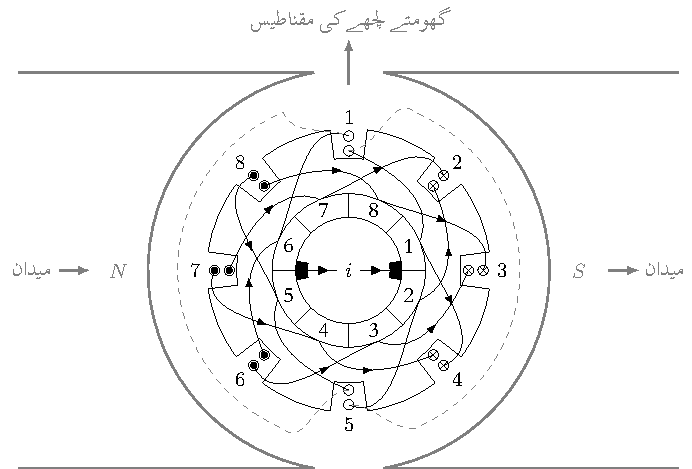
\includegraphics[scale=0.75]{figDCeightTeethCommutatorShortingAcoil}
\begin{tikzpicture}[scale=0.75]
\tikzset{->-/.style={decoration={
  markings,
  mark=at position .5 with {\arrow{latex}}},postaction={decorate}}}
\tikzset{-<-/.style={decoration={
  markings,
  mark=at position .5 with {\arrowreversed{latex}}},postaction={decorate}}}
%grid
%\draw[] (-\tR,-\tR) grid (\tR,\tR);
%
\pgfmathsetmacro{\rR}{2.4}   %stator inner radius
\pgfmathsetmacro{\tR}{\rR+0.2}
\pgfmathsetmacro{\delSlotTheta}{15}   %slot width in degrees
\pgfmathsetmacro{\delR}{0.5}     %slot radial depth
%
\commutator{8}{0}
\foreach \thetaA/\txt in {22.5/2,67.5/1,112.5/8,157.5/7,202.5/6,247.5/5,292.5/4,337.5/3}{\draw node at (\thetaA+22.5:\tR){$\txt$};}
%commutator teeth
\pgfmathsetmacro{\rA}{0.9}
\pgfmathsetmacro{\rB}{1.3}
\pgfmathsetmacro{\rAB}{0.5*(\rA+\rB)}
\draw (0,0) circle (\rA);
\draw (0,0) circle (\rB);
\foreach \thetaA/\txt in {22.5/2,67.5/1,112.5/8,157.5/7,202.5/6,247.5/5,292.5/4,337.5/3}{ \draw (\thetaA+22.5:\rA)--(\thetaA+22.5:\rB); \draw node at (\thetaA+22.5-67.5:\rAB){\txt};}
%bush
\draw[fill](-10:\rA) arc (-10:10:\rA)--++(10:-0.2) arc (10:-10:\rA-0.2) --cycle;
\draw[fill](170:\rA) arc (170:190:\rA)--++(190:-0.2) arc (190:170:\rA-0.2) --cycle;
\draw[] (180:\rA-0.2) to [short,i={$$}] (-0.2,0);
\draw (0.2,0)to [short,i={$$}] (0:\rA-0.2);
\draw[fill=white] node at (0,0){$i$};
%dots
\foreach \thetaA in {112.5,157.5,202.5}{
\draw (\thetaA+22.5:\rR-\delR/4) circle (2.5pt);
\draw[fill] (\thetaA+22.5:\rR-\delR/4) circle (1.5pt);
\draw (\thetaA+22.5:\rR-3*\delR/4) circle (2.5pt);
\draw[fill] (\thetaA+22.5:\rR-3*\delR/4) circle (1.5pt);  } 

\draw (247.5+22.5:\rR-\delR/4) circle (2.5pt);
\draw (247.5+22.5:\rR-3*\delR/4) circle (2.5pt);
%cross
\foreach \thetaA in {22.5,292.5,337.5}{
\draw (\thetaA+22.5:\rR-\delR/4) circle (2.5pt);
\draw (\thetaA+22.5:\rR-\delR/4)++(45:2.2pt)--++(-135:4.4pt);
\draw (\thetaA+22.5:\rR-\delR/4)++(-45:2.2pt)--++(135:4.4pt); 
\draw (\thetaA+22.5:\rR-3*\delR/4) circle (2.5pt);
\draw (\thetaA+22.5:\rR-3*\delR/4)++(45:2.2pt)--++(-135:4.4pt);
\draw (\thetaA+22.5:\rR-3*\delR/4)++(-45:2.2pt)--++(135:4.4pt);}

\draw (67.5+22.5:\rR-\delR/4) circle (2.5pt);
\draw (67.5+22.5:\rR-3*\delR/4) circle (2.5pt);
%arcs to inner side
\foreach \thetaA in {22.5,292.5,337.5}{
\draw[->-] (\thetaA+22.5-67.5:\rB) to [out=\thetaA,in=\thetaA-90] (\thetaA+22.5:\rR-3*\delR/4);    %to inner crosses
\draw[->-] (\thetaA+22.5+67.5:\rB) to [out=\thetaA,in=\thetaA+90] (\thetaA+22.5:\rR-\delR/4);}     %to outer crosses
\def\thetaA{67.5}
\draw[] (\thetaA+22.5-67.5:\rB) to [out=\thetaA,in=\thetaA-90] (\thetaA+22.5:\rR-3*\delR/4);    %to inner crosses
\draw[] (\thetaA+22.5+67.5:\rB) to [out=\thetaA,in=\thetaA+90] (\thetaA+22.5:\rR-\delR/4);
%
\foreach \thetaA in {112.5,157.5,202.5}{
\draw[-<-] (\thetaA+22.5-67.5:\rB) to [out=\thetaA,in=\thetaA-90] (\thetaA+22.5:\rR-3*\delR/4);   %to inner dots
\draw[-<-] (\thetaA+22.5+67.5:\rB) to [out=\thetaA,in=\thetaA+90] (\thetaA+22.5:\rR-\delR/4);}    %to outer dots
\def\thetaA{247.5}
\draw[] (\thetaA+22.5-67.5:\rB) to [out=\thetaA,in=\thetaA-90] (\thetaA+22.5:\rR-3*\delR/4);    %to inner crosses
\draw[] (\thetaA+22.5+67.5:\rB) to [out=\thetaA,in=\thetaA+90] (\thetaA+22.5:\rR-\delR/4);
%gray arc showing back connections
\draw[,dashed] (67.5+22.5:\rR-3*\delR/4) to [out=0,in=135] (45+22.5:\rR+0.5) arc  (45+22.5:-90+22.5:\rR+0.5) to [out=180,in=0] (-112.5+22.5:\rR-\delR/4);
\draw[,dashed] (-112.5+22.5:\rR-3*\delR/4) to [out=180,in=-45] (-135+22.5:\rR+0.5) arc  (-135+22.5:-270+22.5:\rR+0.5) to [out=-67.5,in=157.5] (-292.5+22.5:\rR-\delR/4);
%external magnet
\pgfmathsetmacro{\sp}{1}
\draw[,thick] (100:\rR+\sp) arc (100:260:\rR+\sp)--++(-5,0);
\draw[,thick](100:\rR+\sp)--++(-5,0);
\draw[,thick] node at (180:\rR+1.5){$N$};
\draw[,thick] (80:\rR+\sp) arc (80:-80:\rR+\sp)--++(5,0);
\draw[,thick](80:\rR+\sp)--++(5,0);
\draw[,thick] node at (0:\rR+1.5){$S$};
%direction of mmf
\draw[,thick,-latex] (90:\rR+0.75)--++(0,0.75)node[above]{\RL{گھومتے لچھے کا مقناطیس}};
\draw[,thick,-latex]  (180:\rR+2.5)node[left]{میدان}--++(0.5,0);
\draw[,thick,-latex]  (0:\rR+2)--++(0.5,0)node[right]{میدان};
\end{tikzpicture}
\caption{کاربن بش سمت کار کے دندوں کو قصر دور کر رہا ہے۔}
\label{شکل_یکسمتی_سمتکار_کے_دندے_کسرے_دور}
\end{figure}

اب  تصور کریں کہ مشین ایک جنریٹر کے طور پر استعمال کی جا رہی ہے جس کو خلاف  گھڑی  بیرونی میکانی طاقت سے گھمایا جا رہا ہے۔سمت کار کے آدھے دانت کے برابر حرکت  کے بعد جنریٹر  شکل \حوالہ{شکل_یکسمتی_سمتکار_کے_دندے_کسرے_دور} میں دکھائے گئے حالت میں ہو گا جہاں  دایاں کاربن بش سمت کار کے پہلے اور دوسرے دانت کو قصر دور جبکہ بایاں کاربن بش  پانچویں اور چھٹے دانت کو قصر دور کرتے ہیں۔یوں پہلے اور پانچویں شگافوں کے لچھے قصر دور ہوں گے جبکہ باقی شگافوں کے لچھوں میں حسب معمول برقی رو ہو گا جو پہلے کی طرح اب بھی ساکن لچھوں کے مقناطیسی دباو کے عمودی  مقناطیسی دباو پیدا کریں گے۔آپ گھومتے لچھوں کے میدان کا رخ دائیں ہاتھ کے قانون سے جان سکتے ہیں۔ بائیں جانب تین شگافوں میں رو صفحہ سے باہر جبکہ دائیں جانب تین شگافوں میں صفحہ کے اندر رخ ہے۔ دائیں ہاتھ کی چار انگلیوں کو انہیں کے رخ گھمائیں۔ انگوٹھا میدان کا رک دے گا۔اس لمحہ کی وضاحت شکل \حوالہ{شکل_یکسمتی_دندے_کسرے_دور}  میں کی گئی ہے۔
\begin{figure}
\centering
%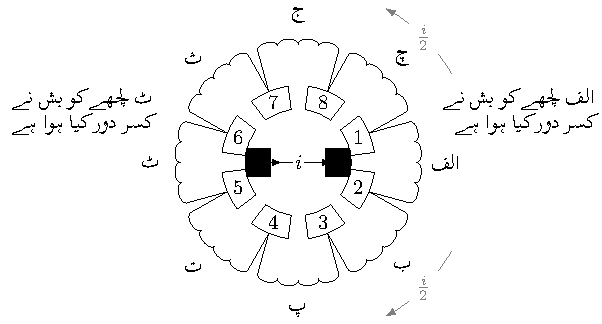
\includegraphics{figDCeightTeethCommutatorShowingCoilConnectionsShortedCoil}
\begin{tikzpicture}
\tikzset{->-/.style={decoration={
  markings,
  mark=at position .5 with {\arrow{latex}}},postaction={decorate}}}
\tikzset{-<-/.style={decoration={
  markings,
  mark=at position .5 with {\arrowreversed{latex}}},postaction={decorate}}}
\pgfmathsetmacro{\rR}{2.4}   %stator inner radius
\pgfmathsetmacro{\tR}{\rR+0.2}
\pgfmathsetmacro{\delSlotTheta}{15}   %slot width in degrees
\pgfmathsetmacro{\delR}{0.5}     %slot radial depth
\pgfmathsetmacro{\rA}{0.9}
\pgfmathsetmacro{\rB}{1.3}
\pgfmathsetmacro{\rC}{2}
\pgfmathsetmacro{\rAB}{0.5*(\rA+\rB)}
\pgfmathsetmacro{\tilt}{22.5}
\pgfmathsetmacro{\delTheta}{30}
%commutator teeth, numbered
\foreach \thetaA/\txt in {0/1,45/8,90/7,135/6,180/5,225/4,270/3,315/2}{
\draw (\thetaA+\tilt-\delTheta/2:\rA) arc (\thetaA+\tilt-\delTheta/2:\thetaA+\tilt+\delTheta/2:\rA)--(\thetaA+\tilt+\delTheta/2:\rB) arc (\thetaA+\tilt+\delTheta/2:\thetaA+\tilt-\delTheta/2:\rB)--cycle;
\draw node at (\thetaA+\tilt:\rAB){$\txt$};  %end of teeth and start of coils
\foreach \i/\j in {0/10,10/20,0/-10,-10/-20}{
\pgfmathsetmacro{\i}{\i+\tilt-22.5}
\pgfmathsetmacro{\j}{\j+\tilt-22.5}
\draw(\thetaA+\i:\rC) to [out=\thetaA+\i,in=\thetaA+\j] (\thetaA+\j:\rC);}
\draw (\thetaA+20+\tilt-22.5:\rC) --(\thetaA+22.5+\tilt-22.5:\rB);
\draw (\thetaA-20+\tilt-22.5:\rC) --(\thetaA-22.5+\tilt-22.5:\rB);  }
%bush
\draw (15:\rA)++(-0.4,0)coordinate (bB);
\draw[fill] (15:\rA) arc (15:-15:\rA)--++(-0.4,0)--(bB) --cycle;
\draw (180+15:\rA)++(0.4,0)coordinate (bA);
\draw[fill] (180+15:\rA) arc (180+15:180-15:\rA)--++(0.4,0)--(bA) --cycle;
%bush current
\draw[->-] (180:\rA-0.4)--++(0.4,0); 
\draw[-<-] (0:\rA-0.4)--++(-0.4,0);
\draw node at (0,0){$i$};
%current
\draw[-latex] (30:\rC+1) arc (30:60:\rC+1);
\draw[-latex] (-30:\rC+1) arc (-30:-60:\rC+1);
\draw (45:\rC+1) node[fill=white]{$\tfrac{i}{2}$};
\draw (-45:\rC+1) node[fill=white]{$\tfrac{i}{2}$};
%text
\draw node at (0+\tilt-22.5:\rC+0.5){ا};
\draw node at (-45+\tilt-22.5:\rC+0.5){ب};
\draw node at (-90+\tilt-22.5:\rC+0.5){پ};
\draw node at (-135+\tilt-22.5:\rC+0.5){ت};
\draw node at (-180+\tilt-22.5:\rC+0.5){ٹ};
\draw node at (-225+\tilt-22.5:\rC+0.5){ث};
\draw node at (-270+\tilt-22.5:\rC+0.5){ج};
\draw node at (-315+\tilt-22.5:\rC+0.5){چ};
\draw node[right,align=right] at (20:\rC+0.5){\RL{لچھا "ا" کو بش نے} \\  \RL{قصر دور کیا ہوا ہے}};
\draw node[left,align=right] at (160:\rC+0.5){\RL{لچھا "ٹ" کو بش نے} \\   \RL{قصر دور کیا ہوا ہے}};
\end{tikzpicture}%
\caption{کاربن بش دو دندوں کو قصر دور کر رہے ہیں۔}
\label{شکل_یکسمتی_دندے_کسرے_دور}
\end{figure}

مشین جب سمت کار کے ایک دانت کے برابر حرکت مکمل کر لے تو کاربن بش دوسرے اور چھٹے دانت سے جڑ جائیں گے۔پہلے اور پانچویں شگافوں میں برقی رو کا رخ پہلے  کے مخالف  ہو جائے گا جبکہ باقی شگافوں میں برقی رو کے رخ برقرار رہیں گے۔گھومتے لچھوں کا برقی دباو اب بھی اسی رخ ہو گا۔

جتنے دورانیہ کے لئے  کاربن بش دو لچھوں کو قصر دور کرتے ہیں اتنے وقت میں ان لچھوں میں برقی رو کا رخ الٹ ہو جاتا ہے۔کوشش کی جاتی ہے کہ  اس دوران برقی رو وقت کے ساتھ بتدریج تبدیل ہو۔ایسا نہ ہونے سے کاربن بش سے چنگاریاں نکلتی ہیں جن سے بش جلد ناکارہ ہو جاتے ہیں۔جنریٹر کے قصر دور لچھوں میں پیدا برقی دباو، قصر دور لچھوں میں گھومتا ناکارہ برقی رو پیدا کرتا ہے جو ہمارے کسی کام کا نہیں ہوتا ہے۔لچھے اور کاربن بش کی  مزاحمت اس ناکارہ  رو کی قیمت تعین کرتے ہیں۔ 

حقیقت میں یک سمت  جنریٹر میں فی قطب درجن دانت کا سمت کار استعمال ہو گا اور اگر مشین بہت چھوٹی نہ ہو تو اس میں دو سے زیادہ قطب ہوں گے۔

%======================
\حصہ{یک سمت  جنریٹر کا برقی دباو}
گزشتہ حصہ کے شکل \حوالہ{شکل_یکسمتی_سمتکار_سے_جڑے_لچھے} میں ا، ب، پ اور ت لچھے سلسلہ وار جڑے ہیں۔ اسی طرح ٹ، ث، ج اور چ لچھے سلسلہ وار جڑے ہیں۔حصہ \حوالہ{حصہ_گھومتے_مشین_محرک_برقی_دباو}  میں مساوات \حوالہ{مساوات_گھومتے_مشین_پیدا_دباو}  یک لچھی یک سمت  جنریٹر کا محرک برقی دباو \عددیء{e_1} دیتی ہے۔ اسے یہاں یاد دھیانی کے لئے دوبارہ پیش کرتے ہیں۔
\begin{align}\label{مساوات_یکسمتی_پیدا_دباو_دوبارہ}
e_1=\omega N \phi_m=\omega N A B_m
\end{align}
خلائی درز میں یکساں \عددیء{B_m} کی صورت میں تمام لچھوں میں ایک جیسا محرک برقی دباو پیدا ہو گا۔یوں شکل \حوالہ{شکل_یکسمتی_سمتکار_بش_کسر_دور_نہیں_کر_رہا}  میں دکھائے لمحہ پر  (شکل \حوالہ{شکل_یکسمتی_سمتکار_سے_جڑے_لچھے} سے رجوع کریں) جنریٹر کا کل محرک برقی دباو \عددیء{e}،  ایک لچھے کے محرک برقی دباو کا چار گنا ہو گا 
\begin{gather}
\begin{aligned}
e&=e_{\textup{ا}}+e_{\textup{ب}}+e_{\textup{پ}}+e_{\textup{ت}}  \\
&=e_{\textup{ٹ}}+e_{\textup{ث}}+e_{\textup{ج}}+e_{\textup{چ}}  \\
&=4 \omega N A B_m
\end{aligned}
\end{gather}
جبکہ شکل \حوالہ{شکل_یکسمتی_سمتکار_کے_دندے_کسرے_دور}  میں دکھائے گئے لمحہ پر \عددی{e} صرف تین لچھوں کے محرک برقی دباو کا مجموعہ ہو گا (شکل \حوالہ{شکل_یکسمتی_دندے_کسرے_دور} سے رجوع کریں):
\begin{gather}
\begin{aligned}
e&=e_{\textup{ب}}+e_{\textup{پ}}+e_{\textup{ت}}  \\
&=e_{\textup{ث}}+e_{\textup{ج}}+e_{\textup{چ}}  \\
&=3 \omega N A B_m
\end{aligned}
\end{gather}
%

\begin{figure}
\centering
%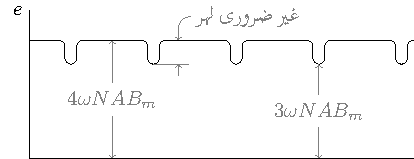
\includegraphics{figDCrippleInVoltage}
\begin{tikzpicture}
\pgfmathsetmacro{\x}{1}
\pgfmathsetmacro{\y}{0.2}
\newcommand{\ripple}{to [out=0,in=90] ++(0.1,-0.1)--++(0,-\y) to [out=-90,in=180]++(0.1,-0.1) to [out=0,in=-90]++(0.1,0.1) --++(0,\y) to [out=90,in=180]++(0.1,0.1)}
%ripple
\draw (0,2)--++(\x/2,0)  \ripple --++(\x,0)  \ripple--++(\x,0)  \ripple--++(\x,0)  \ripple--++(\x,0)  \ripple;  
%axis
\draw (0,0)--(0,2.5) node[left]{$e$};
\draw (0,0)--(6.5,0);
%
\draw[<->] (1.4,0)--++(0,2)node[pos=0.5,fill=white]{$4 \omega N A B_m$};
\draw[<->] (4.9,0)--++(0,1.6)node[pos=0.5,fill=white]{$3 \omega N A B_m$};
\draw[] (2.2,1.6)--++(0.6,0)coordinate[pos=0.7](ripA);
\draw[<-] (ripA)--++(0,-0.2);
\draw[,<-] (ripA)++(0,0.4)--++(0,0.2) to [out=90,in=180] ++(0.2,0.2) node[right]{\RL{غیر مطلوبہ  لہر}};
\end{tikzpicture}
\caption{آٹھ دندی میکانی سمت کار سے حاصل برقی دباو۔}
\label{شکل_یکسمتی-آٹھ_دندوں_سمتکار_کی_لہر}
\end{figure}

شکل \حوالہ{شکل_یکسمتی-آٹھ_دندوں_سمتکار_کی_لہر}  میں آٹھ دندی میکانی سمت کار سے حاصل برقی دباو دکھایا گیا ہے جہاں  یک سمت  برقی دباو پر سوار غیر مطلوبہ  لہر نظر آ رہی ہیں۔اگر جنریٹر  کے ایک جوڑی قطبین پر \عددیء{n} لچھے ہوں تب شکل \حوالہ{شکل_یکسمتی_سمتکار_سے_جڑے_لچھے}  کی طرح یہ دو \عددیء{\tfrac{n}{2}}  سلسلہ وار لچھوں جتنا محرک برقی دباو پیدا کرے گا۔
\begin{align}\label{مساوات_یکسمتی_پیدا_دباو_الف}
e=\frac{n}{2} \omega N \phi_m=\frac{n}{2} \omega N A B_m
\end{align}
اس صورت میں  غیر مطلوبہ لہر کل یک سمت  برقی دباو کی تقریباً
\begin{align}\label{مساوات_یکسمتی_فی_صد_لہر}
\frac{\omega N \phi_m}{\frac{n}{2} \omega N \phi_m} \times 100=\frac{2}{n} \times 100
\end{align}
فی صد ہو گی۔یوں فی قطب دندوں کی تعداد بڑھانے سے زیادہ ہموار برقی دباو حاصل ہو گا اور غیر مطلوبہ لہر قابل نظر انداز ہو گی۔

تصور کریں کہ شکل \حوالہ{شکل_یکسمتی_سمتکار_بش_کسر_دور_نہیں_کر_رہا}  کی مشین کی خلائی درز میں \عددیء{B_m} غیر  یکساں  ہے۔اب لچھوں میں محرک برقی دباو مساوات \حوالہ{مساوات_یکسمتی_پیدا_دباو_دوبارہ}  کے تحت مختلف زاویوں پر مختلف ہو گا۔اس طرح مشین سے حاصل کل برقی دباو چار سلسلہ وار لچھوں کے مختلف محرک برقی دباو کا مجموعہ 
\begin{align} \label{مساوات_یکسمتی_کل_دباو_مجموعہ}
e=e_1+e_2+e_3+e_4
\end{align}
ہو گا جہاں  \عددیء{e_1,e_2,\cdots} مختلف لچھوں کے محرک برقی دباو  ہیں۔
%%%%%%%%%%%%%%%%%%%%%%%%%%%%%%%%

شکل  \حوالہ{شکل_یکسمتی_سمتکار_بش_کسر_دور_نہیں_کر_رہا} میں  گھومتے حصہ کو ایک دندان کے برابر حرکت دینے سے  دوبارہ یہی شکل حاصل ہوتا ہے  لہٰذا ایک دندان حرکت کے بعد حاصل برقی دباو بھی دوبارہ وہی ہو گا۔میکانی سمت کار کے فی قطب دندوں کی تعداد بڑھانے  سے ایک دندان کے برابر حرکت بہت چھوٹی ہو گی لہٰذا خلائی درز میں ہمواری کے ساتھ تبدیل ہوتے کثافت مقناطیسی بہاو کی صورت میں اتنی کم حرکت کے احاطے میں \عددیء{B_m} کی قیمت میں تبدیلی قابل نظر انداز ہو گی اور \عددی{B_m} کو یکساں تصور کیا جا سکتا ہے۔یوں اگر لچھا ایک دندان کے احاطے میں حرکت کرے تو اس میں محرک برقی دباو تبدیل نہیں ہو گا۔یعنی جس لچھے کا محرک برقی دباو  \عددیء{e_1} ہو اس لچھے کا  محرک برقی دباو ایک دندان احاطے میں یہی رہے گا۔یوں اگرچہ \عددیء{e_1,e_2,\cdots} ایک دوسرے سے مختلف ہو سکتے ہیں لیکن ان میں سے ہر ایک کی ایک مستقل قیمت ہو گی، لہٰذا  مساوات \حوالہ{مساوات_یکسمتی_کل_دباو_مجموعہ}  میں دیا گیا محرک برقی دباو (جو ان مستقل قیمتوں کا مجموعہ ہو گا) بھی ایک مستقل ہو گا۔ 


ہم نے دیکھا کہ خلائی درز میں  ہمواری کے ساتھ تبدیل  ہوتے \عددیء{B_m} کی صورت میں جنریٹر سے معیاری یک سمت  محرک برقی دباو حاصل ہو گا۔بدلتا رو جنریٹر میں \عددیء{B_m} سائن نما رکھنا ضروری ہوتا ہے۔نہایت چھوٹی یک سمت  مشینوں کے خلائی درز میں \عددیء{B_m}  یکساں رکھا جاتا ہے جبکہ بڑی مشینوں میں اسے ہمواری کے ساتھ تبدیل کیا جاتا ہے۔جیسا اوپر ذکر ہوا عملاً میکانی سمت کار کے دندوں تک لچھوں کے سروں کی رسائی ممکن تب ہوتی ہے جب ہر شگاف میں دو لچھے رکھے جائیں۔

شگافوں کی تعداد \عددی{n} ہونے کی صورت میں شگافوں کی جوڑیوں کی تعداد \عددی{\tfrac{n}{2}} ہو گی۔ شگافوں کی ایک جوڑی میں \عددی{2} لچھے پائے جاتے ہیں لہٰذا لچھوں کی کل تعداد \عددی{n} ہو گی۔ اگر تمام لچھوں میں ملا کر \عددی{N} چکر ہوں تب ایک لچھے میں \عددی{\tfrac{N}{n}}  چکر ہوں گے اور ایک شگاف کے دو لچھے،  مقناطیسی میدان میں \عددی{\tfrac{2NI}{n}}  کی تبدیلی پیدا کریں گے۔یوں  بالکل قریب قریب شگافوں میں رکھے گئے لچھوں سے خلائی درز میں  سیڑھی نما مقناطیسی دباو کی موج پیدا ہو گی جہاں ہر سیڑھی کی اونچائی  \عددی{\tfrac{2NI}{n}} ہو گی۔ کل چکر  \عددی{N} کو اٹل رکھتے ہوئے شگافوں کی تعداد بڑھانے سے  ایک سیڑھی کی اونچائی کم ہو گی۔  یوں کافی زیادہ شگافوں کی صورت میں ایک سیڑھی کی اونچائی قابل نظر انداز ہو گی اور مقناطیسی موج  کو سیڑھی موج کی بجائے آری کے دندوں کی مانند موج تصور کیا جا سکتا ہے  جسے شکل \حوالہ{شکل_یکسمتی_آری_دندوں_نما_دباو}  میں دکھایا گیا ہے۔  شگافوں میں رو کے رخ کو نقطوں اور صلیبوں سے ظاہر کیا گیا ہے۔ زیادہ تعداد کے شگافوں کی  صورت میں انفرادی لچھوں میں رو کو برقی رو کی چادر تصور کیا جا سکتا ہے۔
\begin{figure}
\centering
%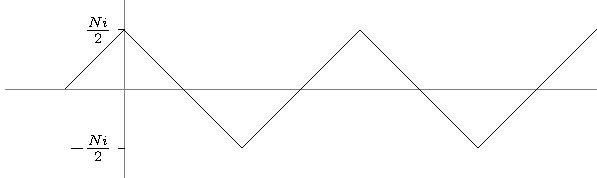
\includegraphics{figDCsawtoothMMF}
\begin{subfigure}{1\textwidth}
\centering
\begin{tikzpicture}
\tikzset{->-/.style={decoration={
  markings,
  mark=at position .5 with {\arrow{latex}}},postaction={decorate}}}
\tikzset{-<-/.style={decoration={
  markings,
  mark=at position .5 with {\arrowreversed{latex}}},postaction={decorate}}}
\pgfmathsetmacro{\rR}{2.4}   %stator inner radius
\pgfmathsetmacro{\tR}{\rR+0.2}
%axis
\draw[gray](-1,0)--(7.5,0);
\draw[gray](0,-1.15)--(0,1.15);
%mmf
\draw(-0.5,-0.5)--++(1.5,1.5)--++(2,-2)--++(2,2)--++(2,-2)--++(0.5,0.5);
\draw (0,1)--++(-0.1,0) node[left] {$\tfrac{Ni}{2}$};
\draw (0,-1)--++(-0.1,0) node[left] {$-\tfrac{Ni}{2}$};
\crossOnly{-0.5,-0.3,-0.1,0.1,0.3,0.5,0.7,0.9,3.1,3.3,3.5,3.7,3.9,4.1,4.3,4.5,4.7,4.9,7.1,7.3,7.5};
\dotOnly{1.1,1.3,1.5,1.7,1.9,2.1,2.3,2.5,2.7,2.9,5.1,5.3,5.5,5.7,5.9,6.1,6.3,6.5,6.7,6.9}
\end{tikzpicture}
\caption{آری دندان مقناطیسی موج اور شگافوں میں رو۔}
\end{subfigure}
\begin{subfigure}{1\textwidth}
\centering
\begin{tikzpicture}
\tikzset{->-/.style={decoration={
  markings,
  mark=at position .5 with {\arrow{latex}}},postaction={decorate}}}
\tikzset{-<-/.style={decoration={
  markings,
  mark=at position .5 with {\arrowreversed{latex}}},postaction={decorate}}}
\pgfmathsetmacro{\rR}{2.4}   %stator inner radius
\pgfmathsetmacro{\tR}{\rR+0.2}
%axis
\draw[gray](-1,0)--(7.5,0);
%current sheet
\draw(-0.5,0.5)--++(1.5,0)--++(0,-1)--++(2,0)--++(0,1)--++(2,0)--++(0,-1)--++(2,0)--++(0,1)--++(0.5,0);
%dots and crosses
\foreach \xLoc in {0.25, 4}{
\draw (\xLoc,0.25) circle (2.5pt);
\draw (\xLoc,0.25)++(45:2.2pt)--++(-135:4.4pt);
\draw (\xLoc,0.25)++(-45:2.2pt)--++(135:4.4pt);} 
\foreach \xLoc in {2,6}{
\draw (\xLoc,-0.25) circle (2.5pt);
\draw[fill] (\xLoc,-0.25) circle (1.5pt); }
\end{tikzpicture}
\caption{شگافوں میں رو کو برقی رو کی چادر تصور کیا گیا ہے۔}
\end{subfigure}
\caption{آری دندوں نما کثافت مقناطیسی دباو۔}
\label{شکل_یکسمتی_آری_دندوں_نما_دباو}
\end{figure}

متعدد قطبین مشین میں شمالی اور جنوبی قطبین کے ایک جوڑے کا پیدا کردہ یک سمت  برقی دباو مساوات \حوالہ{مساوات_یکسمتی_پیدا_دباو_الف}  دے  گی جہاں   قطبین کے ایک جوڑے پر میکانی سمت کار کے دندوں کی تعداد \عددیء{n} ہے۔قطبین کے زیادہ جوڑیوں سے حاصل یک سمت  برقی دباو کو سلسلہ وار یا متوازی جوڑا جا سکتا ہے۔

\حصہ{قوت مروڑ}
یک سمت  مشینوں کا امالی برقی دباو اور قوت مروڑ خلائی درز میں مقناطیسی دباو کی صورت پر منحصر نہیں ہوتا ہے۔

 قوی لچھے کے آری دندان نما مقناطیسی دباو (شکل \حوالہ{شکل_یکسمتی_آری_دندوں_نما_دباو})   کا بنیادی فوریئر جزو\فرہنگ{فوریئر}\حاشیہب{fundamental Fourier component} درج ذیل ہو گا۔
\begin{align}
\tau_q=\frac{8}{\pi^2} \frac{N I}{2}
\end{align}
یک سمت  مشین میں ساکن اور گھومتے لچھوں کے مقناطیسی دباو آپس میں عمودی ہوتے ہیں لہٰذا ان میں قوت مروڑ مساوات \حوالہ{مساوات_گھومتے_مشین_مروڑ_اور_بہاو}  کے تحت درج ذیل ہو گا۔
\begin{align}\label{مساوات_یکسمتی_مروڑ}
T=-\frac{\pi}{2}\left( \frac{P}{2}\right)^2 \phi_m \tau_q 
\end{align} 
%
\ابتدا{مثال}
دو قطب، بارہ دندی میکانی سمت کار کے یک سمت  جنریٹر میں ہر قوی لچھا بیس چکر کا ہے۔ایک لچھے سے \عددیء{0.0442} ویبر  مقناطیسی بہاو گزرتا    ہے۔جنریٹر \عددیء{3600} چکر فی منٹ کی رفتار سے گھوم رہا ہے۔
\begin{itemize}
\item
جنریٹر کے یک سمت  برقی دباو میں غیر مطلوبہ لہر کل برقی دباو کا کتنا فی صد ہو گا؟
\item
یک سمت  برقی دباو حاصل کریں۔
\end{itemize}

حل:
\begin{itemize}
\item
مساوات \حوالہ{مساوات_یکسمتی_فی_صد_لہر}  سے غیر مطلوبہ لہر \عددیء{\tfrac{2}{n} \times 100=\tfrac{2}{12}\times 100=16.66} فی صد حاصل ہوتا ہے۔
\item
جنریٹر کی رفتار \عددیء{\tfrac{3600}{60}=60} ہرٹز ہے یوں مساوات \حوالہ{مساوات_یکسمتی_پیدا_دباو_الف}  سے یک سمت  برقی دباو درج ذیل حاصل ہو گا۔
\begin{align*}
e=\frac{12}{2} \times 2 \times \pi \times 60 \times 20 \times 0.0442=\SI{1999.82}{\volt}
\end{align*}
\end{itemize}
\انتہا{مثال}
%
\حصہ{بیرونی ہیجان  اور خود ہیجان یک سمت  جنریٹر}
\اصطلاح{بیرونی ہیجان}\فرہنگ{ہیجان!بیرونی}\حاشیہب{separately excited}\فرہنگ{separately excited} یک سمت  جنریٹر کے میدانی لچھے کو بیرونی یک سمت  برقی دباو فراہم کیا جاتا ہے جبکہ \اصطلاح{خود ہیجان}\فرہنگ{ہیجان!خود}\حاشیہب{self excited}\فرہنگ{self excited} یک سمت  جنریٹر کے میدانی لچھے کو جنریٹر کا اپنا (قوی لچھے کا) محرک برقی دباو فراہم کیا جاتا ہے۔یک سمت  جنریٹر کی کارکردگی اس کو ہیجان کرنے کے طریقے پر منحصر ہوتی ہے۔
\begin{figure}
\centering
%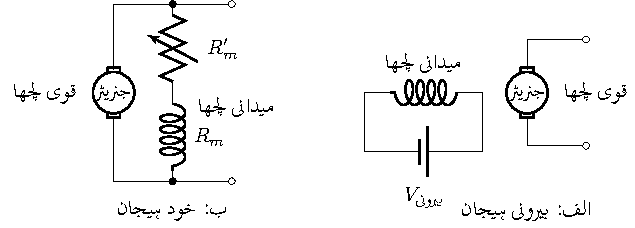
\includegraphics{figDCselfExcitedAndSeparatelyExcited}
\begin{subfigure}{0.45\textwidth}
\centering
\begin{tikzpicture}
\draw (0,0)coordinate(k);
\mymotor{k}{90}{جنریٹر}
\draw (0,0.4)--++(0,0.5) to [short,-o]++(1,0);
\draw (0,-0.4)--++(0,-0.5) to [short,-o]++(1,0);
%field
\draw (-0.75,0) to [inductor]++(-2,0)--++(0,-1) to [battery1,l_={$V_{\textup{بیرونی}}$}]++(2,0) --++(0,1);
\draw node[right] at (0.5,0){\RL{قوی لچھا}};
\draw node at (-1.75,0.5){\RL{میدانی لچھا}};
\end{tikzpicture}
\caption{بیرونی ہیجان}
\end{subfigure}\hfill
\begin{subfigure}{0.45\textwidth}
\centering
\begin{tikzpicture}
\draw (0,0)coordinate(k);
\mymotor{k}{90}{جنریٹر}
\draw (0,0.4)--++(0,1.1) to [short,-o]++(2,0);
\draw (0,-0.4)--++(0,-1.1) to [short,-o]++(2,0);
\draw (1,1.5) to [vR,*-,l={$R_m'$}]++(0,-1.5) to [inductor,l={$R_m$},-*]++(0,-1.5);
\draw node[left] at (-0.5,0){\RL{قوی لچھا}};
\draw node[right] at (1.3,-0.25){\RL{میدانی لچھا}};
\end{tikzpicture}
\caption{ خود ہیجان}
\end{subfigure}%
\caption{بیرونی ہیجان اور خود ہیجان یک سمت  رو جنریٹر۔}
\label{شکل_یکسمتی_خود_ہیجان_بیرونی_ہیجان}
\end{figure}

شکل \حوالہ{شکل_یکسمتی_خود_ہیجان_بیرونی_ہیجان}-ا میں قوی لچھے\فرہنگ{قوی لچھے}\حاشیہب{armature coil}\فرہنگ{armature coil} اور میدانی لچھے\فرہنگ{میدانی لچھے}\حاشیہب{field coil}\فرہنگ{field coil} کو آپس میں عمودی بنایا گیا ہے۔یوں یاد رہتا ہے کہ ان لچھوں کے پیدا کردہ مقناطیسی دباو آپس میں عمودی ہیں۔یہاں قوی لچھے کی صورت میکانی سمت کار کی طرح بنائی گئی ہے۔

میدانی اور قوی لچھوں کے مقناطیسی دباو آپس میں عمودی ہیں جس سے ہم اخذ کر سکتے ہیں کہ ایک لچھے کا برقی دباو دوسرے لچھے کے برقی دباو پر اثر انداز نہیں ہو گا۔یوں مقناطیسی قالب کے کسی ایک رخ  سیرابیت، اس رخ کے عمودی دوسرے رخ کی سیرابیت پر اثر انداز نہیں ہو گی۔

\begin{figure}
\centering
%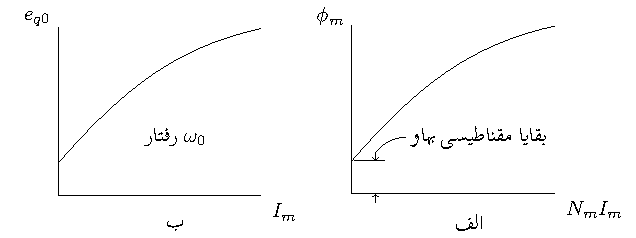
\includegraphics[width=\linewidth]{figDCBrillouinFunctionGeneratedVoltageVersusFieldCurrent}
\pgfmathsetmacro{\J}{0.5}
\pgfmathsetmacro{\k}{(2*\J+1)/(2*\J)}
\begin{subfigure}{0.45\textwidth}
\centering
\begin{tikzpicture}[scale=0.5,
  declare function={
    kBJ(\x)= and(\x>-0.001, \x< 0.001)*(0)+or(\x<-0.001, \x>0.001)*(0.1+\k*(e^(\k*\x)+e^(-\k*\x))/(e^(\k*\x)-e^(-\k*\x))-1/(2*\J)*(e^(\x/(2*\J))+e^(-\x/(2*\J)))/(e^(\x/(2*\J))-e^(-\x/(2*\J))));
kcoth(\x)=(e^\x+e^-\x)/(e^\x-e^-\x);
  }
]
\begin{axis}[
  axis x line=middle, axis y line=middle,
,axis line style={-},
  ymin=0, ymax=1, ytick={0,...,1}, 
ticks=none,
xlabel style={below right},
 ylabel style={above left},
]
\addplot[ domain=0.1:2]{kBJ(x)};
\end{axis}
\draw[] (0.1,1.1)--++(1,0)coordinate[pos=0.7](kk);
\draw[<-](kk)--++(0,0.3) to [out=45,in=180] ++(1,0.5)node[right]{\RL{باقی مقناطیسی بہاو}};
\draw[<-](kk)++(0,-1.1)--++(0,-0.3);
\draw node[below right] at (7,0){$N_mI_m$};
\draw node[left] at (0,6){$\phi_m$};
\end{tikzpicture}
\caption{}
\end{subfigure}\hfill
\begin{subfigure}{0.45\textwidth}
\centering
\begin{tikzpicture}[scale=0.5,
  declare function={
    kBJ(\x)= and(\x>-0.001, \x< 0.001)*(0)+or(\x<-0.001, \x>0.001)*(0.1+\k*(e^(\k*\x)+e^(-\k*\x))/(e^(\k*\x)-e^(-\k*\x))-1/(2*\J)*(e^(\x/(2*\J))+e^(-\x/(2*\J)))/(e^(\x/(2*\J))-e^(-\x/(2*\J))));
  }
]
\begin{axis}[
  axis x line=middle, axis y line=middle,
,axis line style={-},
  ymin=0, ymax=1, ytick={0,...,1}, 
ticks=none,
  %xmin=-5, xmax=5, xtick={-5,...,5}, 
xlabel style={below right},
 ylabel style={above left},
]
\addplot[ domain=0.1:2]{kBJ(x)};
\end{axis}
\draw[] (0.1,1.1)--++(1,0)coordinate[pos=0.7](kk);
\draw[<-](kk)--++(0,0.3) to [out=45,in=180] ++(1,0.5)node[right]{\RL{باقی برقی دباو}};
\draw[<-](kk)++(0,-1.1)--++(0,-0.3);
\draw node at (5,3.5){\RL{رفتار} $\omega_0$};
\draw node[below right] at (7,0){$I_m$};
\draw node[left] at (0,6){$e_{q0}$};
\end{tikzpicture}%
\caption{}
\end{subfigure}%
\caption{میدانی برقی رو سے محرک برقی دباو قابو کیا جاتا ہے۔}
\label{شکل_یکسمتی_پیدا_برقی_دباو_بالمقابل_میدانی_رو}
\end{figure}
شکل \حوالہ{شکل_یکسمتی_خود_ہیجان_بیرونی_ہیجان}-ا میں بیرونی ہیجان مشین کے میدانی لچھے کو بیرونی یک سمت  برقی طاقت مہیا کی گئی ہے۔میدانی لچھے کا برقی رو تبدیل کر کے میدانی مقناطیسی دباو  \عددیء{\tau_m}، میدانی مقناطیسی بہاو \عددیء{\phi_m}  اور کثافت مقناطیسی بہاو \عددیء{B_m}  تبدیل کیے جا سکتے ہیں۔یوں جنریٹر کا محرک برقی دباو مساوات \حوالہ{مساوات_یکسمتی_پیدا_دباو_دوبارہ}  کے تحت تبدیل کیا جا سکتا ہے یا  موٹر کی قوت مروڑ مساوات \حوالہ{مساوات_یکسمتی_مروڑ}  کے تحت تبدیل کی جا سکتی ہے۔

برقی رو کے بڑھنے سے قالب کی سیرابیت  شکل \حوالہ{شکل_یکسمتی_پیدا_برقی_دباو_بالمقابل_میدانی_رو}  میں واضح ہے۔ قالبی سیرابیت کی بنا برقی رو بڑھاتے ہوئے ابتدائی طور محرک برقی دباو اور میدانی لچھے کا برقی رو  راست متناسب ہوں گے جبکہ زیادہ برقی رو پر ایسا نہیں ہو گا۔شکل-ب کی ترسیم مشین کے کھلے سر معائنہ سے حاصل کی جا سکتی ہے۔ شکل-ب میں محرک برقی دباو کو \عددیء{e} کی بجائے  \عددیء{e_{q0}} لکھ کر  یاد دھیانی کرائی گئی ہے  یہ  دباو  قوی لچھے سے  ایک معین رفتار \عددیء{\omega_0} پر حاصل کیا گیا ہے۔کسی دوسری رفتار \عددیء{\omega} پر محرک برقی دباو \عددیء{e_q} کے حصول کے لئے   مساوات \حوالہ{مساوات_یکسمتی_پیدا_دباو_الف} کی مدد  سے 
\begin{align}\label{مساوات_یکسمتی_اندرونی_دباو_بالمقابل_رفتار}
\frac{e_q}{e_{q0}}=\frac{\frac{n}{2} \omega N A B_m}{\frac{n}{2} \omega_0 N A B_m}=\frac{\omega}{\omega_0}
\end{align}
لکھ کر
\begin{align}
e_q=\frac{\omega}{\omega_0}e_{q0}
\end{align}
 یا
\begin{align}\label{مساوات_یکسمتی_چکر_بالمقابل_رفتار}
e_q=\frac{rpm}{rpm_0} e_{q0}
\end{align}
حاصل کیا جا سکتا ہے جہاں رفتار کو چکر فی منٹ\حاشیہب{rpm, rounds per minute} میں (بھی) لیا گیا ہے۔یاد رہے کہ یہ مساوات صرف اس صورت  درست ہوں گے جب مقناطیسی میدان تبدیل نہ ہو۔

شکل \حوالہ{شکل_یکسمتی_خود_ہیجان_بیرونی_ہیجان}-ب میں خود ہیجان مشین دکھائی گئی ہے جس کے میدانی اور قوی لچھے متوازی جڑے ہیں۔ اس طرح جڑے جنریٹر کو \اصطلاح{خود ہیجان  متوازی جڑا}\فرہنگ{داخلی ہیجان!متوازی}\حاشیہب{parallel connected}\فرہنگ{parallel connected} جنریٹر کہتے ہیں۔میدانی لچھے کے ساتھ ایک مزاحمت سلسلہ وار جڑی ہے۔ اس مزاحمت  کو تبدیل کر کے میدانی برقی رو تبدیل کیا جاتا ہے جس سے،بالکل بیرونی ہیجان مشین کی طرح، جنریٹر کا محرک برقی دباو یا موٹر کی قوت مروڑ تبدیل کی جاتی ہے۔
\begin{figure}
\centering
%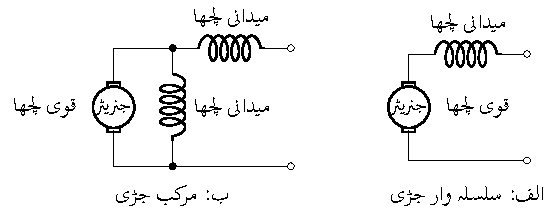
\includegraphics{figDCseriesAndCompound}
\begin{subfigure}{0.45\textwidth}
\centering
\begin{tikzpicture}
\draw (0,0)coordinate(k);
\mymotor{k}{90}{جنریٹر}
\draw (0,0.4)--++(0,0.5) to [inductor,-o,l={\RL{میدانی لچھا}}] ++(2,0);
\draw (0,-0.4)--++(0,-0.5) to [short,-o]++(2,0);
%field
\draw node[right] at (0.5,0){\RL{قوی لچھا}};
\end{tikzpicture}
\caption{سلسلہ وار جڑا}
\end{subfigure}%
\begin{subfigure}{0.45\textwidth}
\centering
\begin{tikzpicture}
\draw (0,0)coordinate(k);
\mymotor{k}{90}{جنریٹر}
\draw (0,0.4)--(0,1)--++(1,0)  to [inductor,-o,l={\RL{میدانی لچھا}}] ++(2,0);
\draw (0,-0.4)--(0,-1) to [short,-o]++(3,0);
\draw (1,1) to [inductor,*-*,l={\RL{میدانی لچھا}}] ++(0,-2);
%field
\draw node[left] at (-0.5,0){\RL{قوی لچھا}};
\end{tikzpicture}
\caption{مرکب جڑا}
\end{subfigure}
\caption{سلسلہ وار اور مرکب جڑا خود ہیجان جنریٹر۔}
\label{شکل_یکسمتی_سلسلہ_وار_اور_مرکب}
\end{figure}
 ایک بار ہیجان ہونے کے بعد مقناطیسی قالب میں  باقی مقناطیسی بہاو رہتا ہے جیسا شکل \حوالہ{شکل_یکسمتی_پیدا_برقی_دباو_بالمقابل_میدانی_رو}-ا میں دکھایا گیا ہے۔یوں میدانی لچھا ہیجان کئے بغیر جنریٹر کچھ  محرک برقی دباو پیدا کرے گا\حاشیہد{آپ ٹھیک سوچ رہے ہیں۔جنریٹر بنانے کے کارخانہ میں قالب کو پہلی مرتبہ مقناطیس بنانا پڑتا ہے ہے۔}۔   شکل-ب میں   صفر میدانی برقی رو پر باقی برقی دباو   دکھایا گیا ہے۔

 خود ہیجان جنریٹر ساکن حال سے چالو ہو کر  ابتدائی طور پر باقی محرک برقی دباو پیدا کرے گا جو میدانی لچھے میں برقی رو پیدا کر کے  مقناطیسی میدان پیدا کرتے ہوئے  مشین کو ذرا زیادہ ہیجان کرتا ہے۔یوں مشین کا محرک برقی دباو بھی کچھ بڑھ جائے گا۔اس طرح کرتے کرتے جنریٹر جلد پورا محرک برقی دباو پیدا کرنا شروع کرتا ہے۔یہ سب اسی دوران  ہوتا ہے جس میں مشین کی رفتار بڑھ رہی ہوتی ہے۔

شکل \حوالہ{شکل_یکسمتی_سلسلہ_وار_اور_مرکب}  میں خود ہیجان جنریٹر کے دو مزید اقسام دکھائے گئے ہیں۔ ایک \اصطلاح{خود ہیجان  سلسلہ وار جڑا} جنریٹر\فرہنگ{داخلی ہیجان!سلسلہ وار}  اور دوسرا \اصطلاح{خود ہیجان  مرکب} جنریٹر\فرہنگ{داخلی ہیجان!مرکب}  ہے۔سلسلہ وار جڑے جنریٹر میں میدانی اور قوی لچھے سلسلہ وار جڑے ہوتے ہیں۔\اصطلاح{مرکب جنریٹر}\فرہنگ{مرکب جنریٹر} میں میدانی لچھا  دو حصوں پر مشتمل ہوتا ہے۔ ایک حصہ قوی لچھے کے متوازی اور دوسرا  سلسلہ وار جڑا ہوتا ہے۔مزید، متوازی  حصہ قوی لچھے کے قریب ہو سکتا ہے یا  سلسلہ وار لچھے کی دوسری جانب، دور جڑا ہو سکتا ہے۔پہلی صورت میں اسے \اصطلاح{قریب جڑا مرکب} جنریٹر\فرہنگ{قریب جڑا مرکب} اور دوسری صورت میں \اصطلاح{دور جڑا مرکب} جنریٹر\فرہنگ{دور جڑا مرکب} کہیں گے۔شکل \حوالہ{شکل_یکسمتی_قریب_دور_جڑی_جنریٹر}  میں مرکب جنریٹر کے دونوں اشکال دکھائے گئے ہیں۔ 
\begin{figure}
\centering
%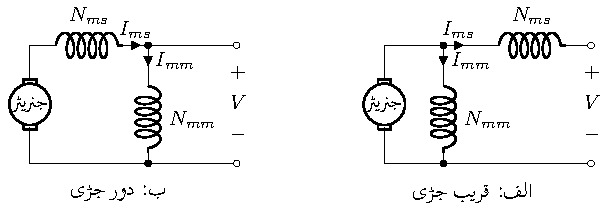
\includegraphics{figDCnearAndFarConnected}
\begin{subfigure}{0.45\textwidth}
\centering
\begin{tikzpicture}
%\draw (0,0)coordinate(k);
%\mymotor{k}{tilt angle}
\draw (0,0)coordinate(k);
\mymotor{k}{90}{جنریٹر}
\draw (0,0.4)--(0,1)--++(1,0)  to  [short,i^={$I_{ms}$}] ++(0.5,0) to [inductor,l={$N_{ms}$},-o]++(2,0);
\draw (0,-0.4)--(0,-1) to [short,-o]++(3.5,0);
\draw (1,1) to [short,*-,i={$I_{mm}$}] ++(0,-0.5) to [inductor,-*,l={$N_{mm}$}]++(0,-1.5);
\draw node at (3.5,0){$\begin{aligned}  &+\\ &V \\ &-  \end{aligned}$};
\end{tikzpicture}
\caption{قریب جڑا}
\end{subfigure}\hfill
\begin{subfigure}{0.45\textwidth}
\centering
\begin{tikzpicture}
\draw (0,0)coordinate(k);
\mymotor{k}{90}{جنریٹر}
\draw (0,0.4)--(0,1)  to [inductor,l={$N_{ms}$},i={$I_{ms}$}]++(2,0)   to [short,-o] ++(1.5,0);
\draw (0,-0.4)--(0,-1) to [short,-o]++(3.5,0);
\draw (2,1) to [short,*-,i={$I_{mm}$}] ++(0,-0.5) to [inductor,l={$N_{mm}$},-*]++(0,-1.5);
\draw node at (3.5,0){$\begin{aligned}  &+\\ &V \\ &-  \end{aligned}$};
\end{tikzpicture}
\caption{دور جڑا}
\end{subfigure}
\caption{مرکب قریب جڑا اور مرکب دور جڑا خود ہیجان جنریٹر}
\label{شکل_یکسمتی_قریب_دور_جڑی_جنریٹر}
\end{figure}

یک سمت  موٹر بھی اسی طرح پکارے جاتے ہیں۔یعنی شکل \حوالہ{شکل_یکسمتی_خود_ہیجان_بیرونی_ہیجان}  کی طرح جڑی دو موٹروں کو بیرونی ہیجان موٹر اور خود ہیجان متوازی جڑی موٹر کہیں گے۔موٹر میں قوی لچھے کا برقی رو جنریٹر کے برقی رو کا مخالف رخ ہو گا۔

تمام اقسام کے یک سمت  جنریٹر کا میدانی مقناطیسی دباو، جنریٹر کے میدانی لچھے کے چکر ضرب برقی رو کے برابر ہو گا:
\begin{align}\label{مساوات_یک_سمت_میدانی_دباو}
\tau=N_m I_m
\end{align}
شکل  \حوالہ{شکل_یکسمتی_خود_ہیجان_بیرونی_ہیجان} میں خود ہیجان متوازی جڑے جنریٹر کے میدانی لچھے میں برقی رو، اس لچھے کی مزاحمت  اور اس کے ساتھ جڑی مزاحمت کے مجموعہ  \عددیء{R=R_m+R_m'} پر منحصر ہو گا یعنی \عددیء{I_m=\tfrac{V}{R}} لہٰذا خود ہیجان متوازی جڑی جنریٹر کے لئے  مساوات \حوالہ{مساوات_یک_سمت_میدانی_دباو}  درج ذیل  صورت اختیار کرتی ہے۔
\begin{align}
\tau_{m,m}=\frac{I_m V}{R_m+R_m'}
\end{align}
سلسلہ وار جڑا جنریٹر میں میدانی برقی رو جنریٹر کے قوی لچھے کا برقی رو ہو گا لہٰذا سلسلہ وار جنریٹر کے لئے مساوات \حوالہ{مساوات_یک_سمت_میدانی_دباو} درج ذیل صورت اختیار کرتی ہے۔
\begin{align}
\tau_{m,s}=N_m I_q
\end{align}
شکل \حوالہ{شکل_یکسمتی_قریب_دور_جڑی_جنریٹر}  کے مرکب جنریٹر میں میدانی مقناطیسی دباو کے دو حصے ہیں۔اس میں \عددیء{N_{mm}} چکر کے متوازی جڑے میدانی لچھے میں برقی رو \عددیء{I_{mm}}  اور  \عددیء{N_{ms}} چکر کے سلسلہ وار جڑے میدانی لچھے میں  برقی رو \عددیء{I_{ms}} ہے لہٰذا اس جنریٹر کے لئے درج ذیل ہو گا۔
\begin{align}
\tau_{m,mk}=N_{ms} I_{ms}+N_{mm} I_{mm}
\end{align}

\حصہ{یک سمت  مشین کی کارکردگی کے خط}
\جزوحصہ{حاصل برقی دباو بالمقابل برقی بوجھ}
مختلف اقسام کے یک سمت  جنریٹروں کے برقی دباو بالمقابل برقی بوجھ خطوط شکل \حوالہ{شکل_یکسمتی_محرک_دباو_بالمقابل_بار}  میں دکھائے گئے ہیں جہاں  گھومتی رفتار اٹل تصور کی گئی ہے۔دھرے پر لاگو بیرونی میکانی طاقت جنریٹر کی قوت مروڑ کے خلاف جنریٹر کو  گھماتی ہے۔
\begin{figure}
\centering
%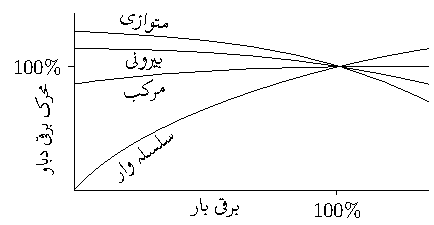
\includegraphics{figDCgeneratedVoltageVersusLoad}
 \newcommand\DrawControl[3]{
  node[#2,circle,fill=#2,inner sep=2pt,label={above:$#1$},label={[black]below:{\footnotesize#3}}] at #1 {}
}
\begin{tikzpicture}[baseline,yscale=0.6]
\draw[] (0,0)--(6,0)node[pos=0.4,below]{\RL{برقی بوجھ}};
\draw[] (0,0)--(0,5);
\node[rotate=90] at (-0.5,1.75){\small\RL{محرک برقی دباو}};
%\draw[help lines] (0,0) grid (8,5);
\draw[] 
  (0,0) .. controls (1,2) and  (4,3.5) .. 
  (6,4);  
\draw node[rotate=35] at (1.2,1){\RL{سلسلہ وار}};
\draw[] 
  (0,3) ..controls(2,3.5) and (4,3.5)..
  (6,3.5) ;  
\draw node[rotate=8] at (1.2,2.8){\RL{مرکب}};
\draw[] 
  (0,4) 
.. controls(2,4) and (4,3.8)..
  (6,3);  
\draw node[rotate=0] at (1.2,3.65){\RL{بیرونی}};
\draw[] 
  (0,4.5) 
.. controls (2,4.3) and (4,4.2)..
  (6,2.5);  
\draw node[rotate=-10] at (1.2,4.75){\RL{متوازی}};
%text
\draw (4.45,0)--++(0,-0.1)node[below]{$\SI{100}{\percent}$};
\draw (0,3.5)--++(-0.1,0)node[left]{$\SI{100}{\percent}$};
\end{tikzpicture}
\caption{یک سمت  جنریٹر کی محرک برقی دباو بمقابلہ برقی بوجھ کے خط۔}
\label{شکل_یکسمتی_محرک_دباو_بالمقابل_بار}
\end{figure}

ان خطوط کو سمجھنے کی خاطر پہلے بیرونی ہیجان جنریٹر پر غور کرتے ہیں جس کا مساوی برقی دور شکل \حوالہ{شکل_یکسمتی_خارجی_ہیجان_کا_مساوی}-ا میں دیا گیا ہے۔بیرونی ہیجان جنریٹر پر برقی بوجھ لادنے سے  قوی لچھے کی مزاحمت\حاشیہد{علامت Rq  کے زیر نوشت میں q لفظ قوی کے پہلی حرف ق کو ظاہر کرتی ہے ۔} \عددیء{R_q} میں  برقی دباو گھٹتا ہے۔یوں جنریٹر سے حاصل برقی دباو \عددیء{V}، جنریٹر کے اندرونی محرک برقی دباو \عددیء{E_q}  سے کچھ کم ہو گا:
\begin{align}
V=E_q-I_q R_q
\end{align}
برقی بوجھ \عددیء{I_q} بڑھانے سے  \عددی{V} مزید کم ہو گا۔بیرونی ہیجان جنریٹر کا خط یہی رجحان ظاہر کرتا ہے۔حقیقت میں دیگر وجوہات بھی اثر انداز ہوتے ہیں جن کی بنا یہ خط سیدھا نہیں بلکہ جھکا ہوتا ہے۔ 
\begin{figure}
\centering
%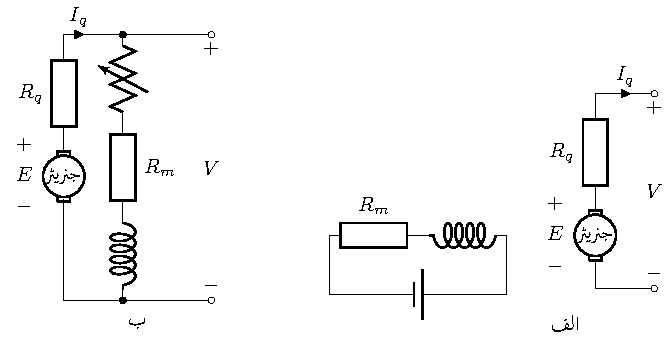
\includegraphics{figDCseparateExcitedEquivalentCircuit}
\begin{subfigure}{0.60\textwidth}
\centering
\begin{tikzpicture}
\draw (0,0)coordinate(k);
\mymotor{k}{90}{جنریٹر}
\draw (-0.7,0) node {$\begin{aligned} &+\\ &E_q\\ &-  \end{aligned}$};
\draw (0,0.4) to [european resistor,l={$R_q$}]++(0,2) to [short,-o,i={$I_q$}]++(1,0)node[below]{$+$};
\draw (0,-0.4)--++(0,-0.5)  to [short,-o]++(1,0)node[above]{$-$};
\draw node at (1,0.75){$  V $};
%
\draw (-1.5,0) to [inductor]++(-1.5,0) to [european resistor,l_={$R_m$}]++(-1.5,0) --++(0,-1) to [battery1]++(3,0)--++(0,1);
\end{tikzpicture}
\caption{}
\end{subfigure}\hfill
\begin{subfigure}{0.30\textwidth}
\centering
\begin{tikzpicture}
\draw (0,0)coordinate(k);
\mymotor{k}{90}{جنریٹر}
\draw (-0.7,0) node {$\begin{aligned} &+\\ &E_q\\ &-  \end{aligned}$};
\draw (0,0.4) to [european resistor,l={$R_q$}]++(0,2) to [short,i={$I_q$}]++(0.5,0) to [short,-o]++(2,0)node(a)[below]{$+$};
\draw (0,-0.4)--++(0,-1.7)  to [short,-o]++(2.5,0)node(b)[above]{$-$};
\draw (1,2.4) to [vR,*-]++(0,-1.5) to [european resistor,l={$R_m$}]++(0,-1.5) to [inductor,-*]++(0,-1.5);
\draw node at ($(a)!0.5!(b)$){$  V $};
\end{tikzpicture}
\caption{}
\end{subfigure}
\caption{بیرونی ہیجان، متوازی جڑے جنریٹر کا مساوی برقی دور۔}
\label{شکل_یکسمتی_خارجی_ہیجان_کا_مساوی}
\end{figure}

متوازی جڑی جنریٹر کے خط کا بھی یہی رجحان ہے۔ متوازی جڑی جنریٹر پر بھی برقی بوجھ لادنے سے قوی لچھے کی مزاحمت میں برقی دباو گھٹتا ہے ۔یوں اس کے میدانی لچھے پر لاگو برقی دباو بھی کم ہو جاتا ہے جس سے میدانی لچھے میں برقی رو گھٹتا ہے۔ اس سے محرک برقی دباو مزید کم ہوتا ہے۔یوں متوازی جڑے جنریٹر کے برقی دباو بالمقابل برقی بوجھ  خط کی ڈھلوان بیرونی ہیجان جنریٹر کی خط سے زیادہ ہو گی۔
\begin{figure}
\centering
%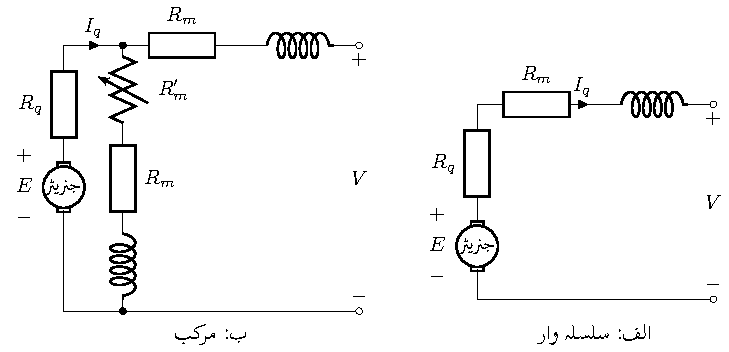
\includegraphics{figDCseriesAndCompoundEquivalentCircuit}
\begin{subfigure}{0.40\textwidth}
\centering
\begin{tikzpicture}
\draw (0,0)coordinate(k);
\mymotor{k}{90}{جنریٹر}
\draw (-0.7,0) node {$\begin{aligned} &+\\ &E_q\\ &-  \end{aligned}$};
\draw (0,0.4) to [european resistor,l={$R_q$}]++(0,2) to [european resistor,l={$R_m$},i={$I_q$}]++(2,0) to [inductor,-o] ++(2,0)node[below]{$+$}coordinate(upper);
\draw (0,-0.4)--++(0,-0.5)  to [short,-o]++(4,0)node[above]{$-$}coordinate(lower);
\draw node at ($(upper)!0.5!(lower)$){$  V $};
\end{tikzpicture}
\caption{سلسلہ وار}
\end{subfigure}\hfill
\begin{subfigure}{0.50\textwidth}
\centering
\begin{tikzpicture}
\draw (0,0)coordinate(k);
\mymotor{k}{90}{جنریٹر}
\draw (-0.7,0) node {$\begin{aligned} &+\\ &E_q\\ &-  \end{aligned}$};
\draw (0,0.4) to [european resistor,l={$R_q$}]++(0,2) to [short,i={$I_q$}]++(1,0)  to [european resistor,l={$R_{m1}$}]++(2,0) to [inductor,-o]++(2,0)node(a)[below]{$+$};
\draw (0,-0.4)--++(0,-1.7)  to [short,-o]++(5,0)node(b)[above]{$-$};
\draw (1,2.4) to [vR,l={$R_m'$},*-]++(0,-1.5) to [european resistor,l={$R_{m2}$}]++(0,-1.5) to [inductor,-*]++(0,-1.5);
\draw node at ($(a)!0.5!(b)$){$  V $};
\end{tikzpicture}
\caption{مرکب}
\end{subfigure}
\caption{سلسلہ وار اور مرکب جنریٹر کے مساوی برقی دور۔}
\label{شکل_یکسمتی_سلسلہ_وار_اور_مرکب_مساوی}
\end{figure}

شکل \حوالہ{شکل_یکسمتی_سلسلہ_وار_اور_مرکب_مساوی}  میں سلسلہ وار اور مرکب جنریٹر کے مساوی برقی ادوار دکھائے گئے ہیں۔سلسلہ وار جڑے جنریٹر کے میدانی لچھے میں لدے  بوجھ کا برقی رو  گزرتا ہے۔اس طرح بوجھ بڑھانے سے میدانی مقناطیسی دباو  بڑھ کر محرک برقی دباو بڑھاتا ہے۔سلسلہ وار جڑے جنریٹر کا خط یہی دکھا رہا ہے۔سلسلہ وار جڑے جنریٹر عموماً استعمال نہیں ہوتے چونکہ ان سے حاصل برقی دباو، بوجھ کے ساتھ بہت زیادہ تبدیل ہوتا ہے۔ 

مرکب جڑے جنریٹر کی کارکردگی سلسلہ وار اور متوازی جڑا جنریٹر کے بیچ ہے۔مرکب جنریٹر میں بوجھ بڑھانے سے قوی لچھے کی وجہ سے حاصل برقی دباو میں کمی کو میدانی لچھے کا بڑھتا مقناطیسی دباو پورا کرتا ہے۔یوں مرکب جنریٹر سے حاصل برقی دباو، لدے بوجھ کے ساتھ بہت کم تبدیل ہوتا ہے۔

بیرونی ہیجان، متوازی اور مرکب جڑے جنریٹر سے حاصل برقی دباو کو متوازی جڑی لچھے کے برقی رو  سے وسیع حدوں تک تبدیل کیا جا سکتا ہے۔

قوی لچھا برقی بوجھ کو درکار برقی رو فراہم کرتا ہے لہٰذا یہ موٹی موصل تار کا بنا اور عموماً کم چکر کا ہوتا ہے۔سلسلہ وار جنریٹر کے میدانی لچھے سے  مشین کا پورا برقی رو  گزرتا ہے لہٰذا یہ بھی موٹی موصل تار کا بنا ہوتا ہے۔باقی مشینوں کے میدانی لچھوں میں پورے برقی بوجھ کا چند  فی صد برقی رو گزرتا ہے لہٰذا یہ باریک موصل تار کے بنائے اور عموماً زیادہ چکر کے ہوتے ہیں۔

\جزوحصہ{رفتار بالمقابل قوت مروڑ}
یہاں بھی شکل \حوالہ{شکل_یکسمتی_خارجی_ہیجان_کا_مساوی}  اور شکل \حوالہ{شکل_یکسمتی_سلسلہ_وار_اور_مرکب_مساوی}  سے رجوع کریں البتہ ان اشکال میں برقی رو کے رخ الٹ کر دیں۔یک سمت  موٹر بھی جنریٹر کی طرح مختلف طریقوں سے جڑے جاتے ہیں۔موٹر کو معین بیرونی برقی دباو دی جاتی ہے جہاں سے یہ برقی رو حاصل کرتا ہے۔برقی رو باہر سے قوی لچھے میں داخل ہوتا ہے لہٰذا ان کے لئے درج ذیل لکھا جا سکتا ہے۔
\begin{gather}
\begin{aligned}\label{مساوات_یکسمتی_دباو_رو_قوی_سلسلہ_وار}
V&=E_q+I_q R_q\\
I_q&=\frac{V-E_q}{R_q}
\end{aligned}
\end{gather}
بیرونی ہیجان اور متوازی جڑی موٹروں میں میدانی لچھے کو برقرار معین بیرونی برقی دباو فراہم کیا جاتا ہے لہٰذا میدانی مقناطیسی بہاو پر میکانی بوجھ کا کوئی اثر نہیں ہوتا ہے۔بڑھتا میکانی بوجھ اٹھانے کی خاطر، مساوات \حوالہ{مساوات_یکسمتی_مروڑ}   کے تحت، قوی لچھے کا مقناطیسی بہاو بڑھنا ہو گا۔یہ تب ممکن ہو گا جب قوی لچھے میں برقی رو بڑھے۔ مساوات \حوالہ{مساوات_یکسمتی_دباو_رو_قوی_سلسلہ_وار}  سے ہم دیکھتے ہیں کہ قوی لچھے کا محرک برقی دباو \عددیء{E_q}  گھٹنے سے  \عددی{I_q} بڑھے گا۔امالی دباو \عددیء{E_q} موٹر کی رفتار پر منحصر ہے   لہٰذا موٹر کی رفتار کم ہو جائے گی (مساوات \حوالہ{مساوات_یکسمتی_پیدا_دباو_الف})۔یوں جیسا  شکل \حوالہ{شکل_یکسمتی_موٹر_رفتار_بالمقابل_بار}   میں  دکھایا گیا ہے میکانی بوجھ بڑھانے سے موٹر کی رفتار کم ہوتی ہے۔
\begin{figure}
\centering
%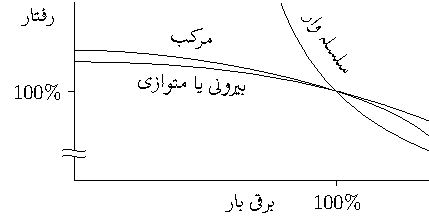
\includegraphics{figDCmotorSpeedVersusLoad}
\newcommand\DrawControl[3]{
  node[#2,circle,fill=#2,inner sep=2pt,label={above:$#1$},label={[black]below:{\footnotesize#3}}] at #1 {}
}
\begin{tikzpicture}[baseline]
\draw[] (0,0)--(6,0);
\node at (3,-0.4) {\RL{میکانی بار}};
\draw[] (0,0)--(0,0.4);
\draw (0,0.5)--(0,3);
\node[left] at (-0.2,2.75){\RL{رفتار}};
%
\draw[]   (0,2) .. controls(2,2) and (4,1.8)..  (6,1);  
\draw node[rotate=-2.5] at (2,1.6){\RL{بیرونی یا متوازی}};
%
\draw[]   (0,2.2) ..controls (2,2.2) and (5,1.6)..  (6,0.75);  
\draw node[rotate=-5] at (2,2.4){\RL{مرکب}};
%
\draw[]   (3.5,3) .. controls (4,1.6) and (5,0.9)  ..(6,0.5);  
\draw node[rotate=-57] at (4.3,2.3){\RL{سلسلہ وار}};
%text
\draw (4.45,0)--++(0,-0.1)node[below]{$\SI{100}{\percent}$};
\draw (0,1.5)--++(-0.1,0)node[left]{$\SI{100}{\percent}$};
%
\draw (-0.2,0.5) to [out=30,in=210] (0.2,0.5);
\draw (-0.2,0.4) to [out=30,in=210] (0.2,0.4);
\end{tikzpicture}%
\caption{یک سمت  موٹر کے میکانی بوجھ بالمقابل رفتار خطوط۔}
\label{شکل_یکسمتی_موٹر_رفتار_بالمقابل_بار}
\end{figure}

متوازی جڑی یا بیرونی ہیجان موٹر تقریباً  مستقل رفتار  برقرار رکھتی ہے۔اس کی رفتار بے بوجھ حالت سے پوری طرح بوجھ بردار حالت تک تقریباً  پانچ فی صد گھٹتی ہے۔ان موٹروں کی رفتار نہایت آسانی سے میدانی لچھے کا برقی رو تبدیل کر کے تبدیل کی جاتی ہے۔میدانی لچھے کے ساتھ سلسلہ وار جڑی مزاحمت تبدیلی کر کے میدانی لچھے کا برقی رو تبدیل کیا جاتا ہے۔یوں ان کی رفتار  وسیع حدوں کے بیچ تبدیل کرنا ممکن ہوتا ہے۔موٹر پر لاگو بیرونی برقی دباو تبدیل کر کے بھی رفتار قابو کی جا سکتی ہے۔ایسا عموماً قوی برقیات کی مدد سے کیا جاتا ہے۔

ساکن حال سے چالو کرتے ہوئے لمحہ کی قوت مروڑ اور  زیادہ سے زیادہ قوت مروڑ، ان موٹروں کے  قوی لچھے تک برقی رو پہنچانے کی صلاحیت پر منحصر ہوتی ہے جو ازخود میکانی سمت کار پر منحصر ہو گا۔

سلسلہ وار جڑی موٹر پر میکانی بوجھ بڑھانے سے  قوی اور میدانی لچھوں میں برقی رو  بڑھتا ہے۔فراہم کردہ دباو  \عددی{V}، مزاحمت  \عددی{R_q} اور \عددی{R_m} اٹل ہونے کی بنا، \عددی{I_q} بڑھانے کی خاطر \عددیء{E_q}  کو کم ہونا ہو گا \عددی{(I_q=\tfrac{V-E_q}{R_m+R_q})} جو موٹر کی رفتار گھٹنے سے ہو گا۔ بڑھتے \عددی{I_q} کی بنا میدانی مقناطیسی بہاو \عددی{\phi_m} بھی بڑھتا ہے لہٰذا  بوجھ بڑھانے سے  موٹر کی رفتار کافی زیادہ کم ہونی ہو گی (مساوات \حوالہ{مساوات_یکسمتی_پیدا_دباو_الف}) ۔ایسی موٹریں ان مقامات پر بہتر ثابت ہوتی ہیں جہاں زیادہ قوت مروڑ درکار ہو۔بڑھتی قوت مروڑ کے ساتھ ان کی رفتار کم ہونے کی وجہ سے  درکار برقی طاقت، قوت مروڑ کے ساتھ زیادہ تبدیل نہیں ہوتی۔

یہاں اس بات کا ذکر ضروری ہے کہ بے بوجھ سلسلہ وار جڑی موٹر کی رفتار خطرناک حد تک بڑھ سکتی ہے۔سلسلہ وار موٹر کو استعمال کرتے وقت اس بات کا خاص خیال رکھنا ضروری ہے کہ موٹر ہر لمحہ بوجھ بردار رہے۔

ساکن  موٹر چالو کرتے وقت   \عددیء{I_q}  زیادہ ہو گا لہٰذا زیادہ  مقناطیسی بہاو پیدا ہو گا۔یوں چالو کرتے وقت موٹر کی قوت مروڑ خاصی زیادہ ہو گی۔ یہ ایک اچھی خوبی ہے جس کی بنا بوجھ بردار ساکن موٹر کو چالو کرنا آسان ہوتا ہے۔

مرکب موٹروں میں ان دو اقسام کی موٹروں کے خواص پائے جاتے ہیں۔جہاں بوجھ بردار موٹر چالو کرنا ضروری ہو لیکن رفتار میں سلسلہ وار موٹر جتنی تبدیلی منظور نہ ہو وہاں مرکب موٹریں کارآمد ثابت ہوتی ہیں۔

\ابتدا{مثال}
ایک \عددیء{75}  کلو واٹ، \عددیء{415} وولٹ اور \عددیء{1200} چکر فی منٹ کی رفتار سے چلنے والی متوازی جڑی یک سمت  موٹر کے قوی لچھے کی مزاحمت \عددیء{0.072} اوہم اور میدانی لچھے کی مزاحمت  \عددیء{83.2} اوہم ہے۔بوجھ بردار موٹر   \عددیء{1123} چکر فی منٹ کی رفتار سے چلتے ہوئے  \عددیء{112} ایمپیئر لے رہی ہے۔ 
\begin{itemize}
\item
میدانی برقی رو اور قوی لچھے کا برقی رو حاصل کریں۔
\item
موٹر کی اندرونی پیدا کردہ برقی دباو حاصل کریں۔
\item
اگر میدانی لچھے کی مزاحمت \عددیء{100.2} اوہم کر دی جائے  لیکن قوی لچھے کا برقی رو تبدیل نہ ہو  تب موٹر کی رفتار کتنی ہو گی؟ قالب کی سیرابیت کو نظرانداز کریں۔
\end{itemize}

\begin{figure}
\centering
%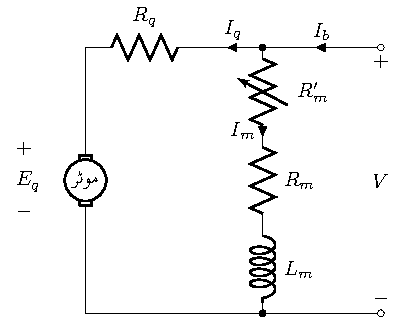
\includegraphics{figDCmotorExample}
\begin{tikzpicture}
\draw (0,0)coordinate(k);
\mymotor{k}{90}{موٹر}
\draw node at (-1,0){$\begin{aligned}  &+ \\   & E_q \\ &-  \end{aligned}$};
\draw (0,0.4)--++(0,1.85) to [resistor,l={$R_q$}] ++(2,0)  to [short,i<={$I_q$}] ++(1,0) to  [short,-o,i<={$I_b$}]++(2,0)node[below](a){$+$};
\draw (0,-0.4)--++(0,-1.85) to [short,-o]++(5,0)node[above](b){$-$};
\draw (3,2.25) to [vR,i_={$I_m$},*-,l={$R_m'$}]++(0,-1.5) to [resistor,l={$R_m$}] ++(0,-1.5)  to [inductor,l={$L_m$},-*]++(0,-1.5);
\draw node at ($(a)!0.5!(b)$){$V$};
\end{tikzpicture}
\caption{یک سمت  موٹر کی مثال۔}
\label{شکل_یکسمتی_موٹر_کی_مثال}
\end{figure}

حل:
\begin{itemize}
\item
شکل \حوالہ{شکل_یکسمتی_موٹر_کی_مثال}  سے رجوع کریں۔\عددیء{415} وولٹ پر میدانی لچھے کا برقی رو درج ذیل ہو گا۔
\begin{align*}
I_m=\tfrac{V}{R_m+R_m'}=\frac{415}{83.2}=\SI{4.988}{\ampere}
\end{align*}
یوں قوی لچھے کا برقی رو \عددیء{I_q=I_b-I_m=112-4.988=\SI{107.012}{\ampere}} ہو گا۔
\item
یک سمت  موٹر کا اندرونی پیدا کردہ برقی دباو درج ذیل ہو گا۔
\begin{align*}
E_q=V-I_q R_q=415-107.012\times 0.072=\SI{407.295}{\volt}
\end{align*}
\item
اگر میدانی لچھے کی مزاحمت \عددیء{100.2} اوہم کر دی جائے  تب \عددی{I_m} درج ذیل ہو گا۔
\begin{align*}
I_m=\frac{V}{R_m+R_m'}=\frac{415}{100.2}=\SI{4.1417}{\ampere}
\end{align*}
\item
اگر قوی لچھے کا برقی رو \عددیء{107.012} ایمپیئر ہی رکھا جائے تب  اندرونی دباو درج ذیل ہو گا۔
\begin{align*}
E_q=V-I_q R_q=415-107.012 \times 0.072=\SI{407.295}{\volt}
\end{align*}
\item
مساوات \حوالہ{مساوات_یکسمتی_پیدا_دباو_الف}  کی مدد سے  چونکہ اندرونی پیدا کردہ برقی دباو تبدیل نہیں ہوا لیکن مقناطیسی بہاو تبدیل ہوا ہے لہٰذا موٹر کی رفتار تبدیل ہو گی۔ان دو مقناطیسی بہاو اور رفتاروں پر مساوات \حوالہ{مساوات_یکسمتی_اندرونی_دباو_بالمقابل_رفتار} کی طرح  درج ذیل لکھا جا سکتا ہے۔
\begin{align*}
\frac{E_{q1}}{E_{q2}}=\frac{\frac{n}{2} \omega_1 N \phi_{m1}}{\frac{n}{2} \omega_2 N \phi_{m2}}
\end{align*}
اب چونکہ \عددیء{E_{q1}=E_{q2}} ہے  لہٰذا \عددیء{\omega_1 \phi_{m1}=\omega_2 \phi_{m2}} ہو گا۔قالبی سیرابیت  نظرانداز کرتے ہوئے مقناطیسی بہاو، میدانی دباو پر منحصر ہو گا جو از خود میدانی برقی رو پر منحصر ہو گا  لہٰذا درج ذیل ہو گا۔
\begin{align*}
\frac{\omega_1}{\omega_2}=\frac{rpm_1}{rpm_2}=\frac{\phi_{m2}}{\phi_{m1}}=\frac{I_{m2}}{I_{m1}}
\end{align*}
یوں  نئی رفتار
\begin{align*}
rpm_2=\frac{I_{m1}}{I_{m2}} \times rpm_1=\frac{4.988}{4.1417} \times 1123=1352.47
\end{align*}
چکر فی منٹ حاصل ہوتی ہے۔اس مثال میں ہم دیکھتے ہیں کہ میدانی برقی رو کم کرنے سے موٹر کی رفتار بڑھتی ہے۔
\end{itemize}
\انتہا{مثال}
%
\ابتدا{مثال}
ایک \عددیء{60} کلو واٹ، \عددیء{415} وولٹ، \عددیء{1000} چکر فی منٹ متوازی جڑی یک سمت  موٹر کی قوی لچھے کی مزاحمت \عددیء{0.05} اوہم  اور میدانی لچھے کی \عددیء{60}  اوہم ہے۔بے بوجھ موٹر کی رفتار \عددیء{1000} چکر فی منٹ ہے۔میدانی لچھا \عددیء{1000} چکر کا ہے۔
\begin{itemize}
\item
جب یہ موٹر  \عددی{70} ایمپیئر  لے رہی ہو اس وقت اس کی رفتار معلوم کریں۔
\item
\عددیء{140} ایمپیئر پر اس کی رفتار معلوم کریں۔
\item
\عددیء{210} ایمپیئر پر اس کی رفتار معلوم کریں۔
\item
اس موٹر کی رفتار بالمقابل قوت مروڑ ترسیم کریں  ۔
\end{itemize}

\begin{figure}
\centering
%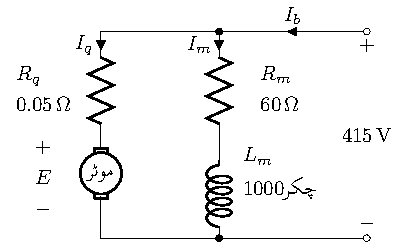
\includegraphics{figDCparallelMotorExample}
\begin{tikzpicture}
\draw (0,0)coordinate(k);
\mymotor{k}{90}{موٹر}
\draw node at (-1,-0.1){$\begin{aligned}  &+ \\   & E_q \\ &-  \end{aligned}$};
\draw (0,0.4) to [resistor,i<={$I_q$}] ++(0,2) --++(2,0)  to  [short,-o,i<={$I_b$}]++(2.5,0)node[below](a){$+$};
\draw (0,-0.4)--++(0,-0.7) to [short,-o]++(4.5,0)node[above](b){$-$};
\draw (2,-1.1)  to [inductor,*-] ++(0,1.5) to [resistor,i<={$I_m$},-*] ++(0,2);
\draw node at ($(a)!0.5!(b)$){$\SI{415}{\volt}$};
%text
\draw node at (-1,1.4){$\begin{aligned}  & R_q \\ &\SI{0.05}{\ohm}  \end{aligned}$};
\draw node at (3,1.4){$\begin{aligned}  & R_m \\ &\SI{60}{\ohm}  \end{aligned}$};
\draw node at (3,0){$\begin{aligned}  & L_m \\ &1000 \textup{چکر}  \end{aligned}$};
\end{tikzpicture}
\caption{متوازی جڑی موٹر کی مثال۔}
\label{شکل_یکسمتی_متوازی_موٹر_کی_مثال}
\end{figure}
%
\begin{figure}
\centering
%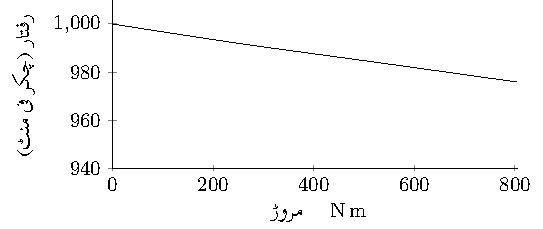
\includegraphics{figDCmotorSpeedVersusTorque}
\newcommand\DrawControl[3]{
  node[#2,circle,fill=#2,inner sep=2pt,label={above:$#1$},label={[black]below:{\footnotesize#3}}] at #1 {}
}
\begin{tikzpicture}
\begin{axis}[yscale=0.5,
ymin=940,
ymax=1010,
%axis lines=middle,
axis x line=bottom,
axis y line=left,
axis line style=-, 
]
    \addplot[smooth] plot coordinates {(0,1000) (250.088,991.95) (527.35,983.96) (804.65,975.83)};
\end{axis}
\draw node at (3.5,-0.75){مروڑ \quad \si{\newton \meter}};
\draw node[rotate=90] at (-1.5,1.4){\RL{رفتار (چکر فی منٹ)}};
\end{tikzpicture}
\caption{رفتار بالمقابل قوت مروڑ۔}
\label{شکل_یکسمتی_رفتار_بالمقابل_مروڑ}
\end{figure}


حل:
\begin{itemize}
\item
شکل \حوالہ{شکل_یکسمتی_متوازی_موٹر_کی_مثال} میں موٹر دکھائی گئی ہے۔متوازی میدانی لچھے کے برقی رو پر بوجھ کا کوئی اثر نہیں ہو گا۔لہٰذا میدانی مقناطیسی بہاو بے بوجھ اور بوجھ بردار موٹر میں ایک جیسا ہو گا۔بے بار یک سمت  موٹر کے قوی لچھے کا برقی رو \عددیء{I_q}  قابل نظر انداز ہوتا ہے۔اس طرح مساوات \حوالہ{مساوات_یکسمتی_دباو_رو_قوی_سلسلہ_وار}  اور مساوات \حوالہ{مساوات_یکسمتی_چکر_بالمقابل_رفتار}  سے  درج ذیل حاصل ہوں گے۔
\begin{align*}
E_q&=V-I_q R_q=415-0\times R_q=\SI{415}{\volt}\\
I_m&=\frac{V}{R_m}=\frac{415}{60}=\SI{6.916}{\ampere}
\end{align*}
یوں \عددیء{415} وولٹ محرک برقی دباو پر  \عددیء{1000} چکر فی منٹ یا \عددیء{16.66} چکر فی سیکنڈ رفتار حاصل ہو گا۔\عددیء{70} ایمپیئر برقی بوجھ پر بھی \عددیء{I_m=\SI{6.916}{\ampere}} ہو گا جبکہ  \عددی{I_q} درج ذیل ہو گا۔
\begin{align*}
I_q=I_b-I_m=70-6.916=\SI{63.086}{\ampere}
\end{align*}
 مساوات \حوالہ{مساوات_یکسمتی_دباو_رو_قوی_سلسلہ_وار}  سے 
\begin{align*}
E_q=V-I_q R_q=415-63.086 \times 0.05=\SI{411.8458}{\volt}
\end{align*}
اور مساوات \حوالہ{مساوات_یکسمتی_چکر_بالمقابل_رفتار}  سے رفتار (چکر فی منٹ) حاصل کرتے ہیں۔
\begin{align*}
rpm=\frac{e_q}{e_{q0}} rpm_0=\frac{411.8458}{415} \times 1000=991.95
\end{align*}
%
\item
آئیں ان تمام کو  \عددیء{I_b=\SI{140}{\ampere}} کے لئے حاصل کریں۔
\begin{align*}
I_q&=I_b-I_m=140-6.916=\SI{133.084}{\ampere}\\
E_q&=415-133.084 \times 0.05=\SI{408.3458}{\volt}\\
rpm&=\frac{408.3458}{415} \times 1000=983.96
\end{align*}
%
\item
یہاں \عددیء{I_b=\SI{210}{\ampere}} ہے لہٰذا درج ذیل ہوں گے۔
\begin{align*}
I_q&=I_b-I_m=210-6.916=\SI{203.084}{\ampere}\\
E_q&=415-203.084 \times 0.05=\SI{404.8458}{\volt}\\
rpm&=\frac{404.8458}{415} \times 1000=975.83
\end{align*}
%
\item
موٹر میں ضیاع طاقت  کو نظر انداز کرتے ہوئے میکانی طاقت فراہم کردہ برقی طاقت کے برابر ہو گی:
\begin{align}
e_q I_q=T \omega
\end{align}
یوں پچھلے جزو سے حاصل جوابات کی مدد سے بے بوجھ موٹر کی قوت مروڑ  صفر ہو گی یعنی \عددیء{T_0=\SI{0}{\newton \meter}}  جبکہ \عددیء{70}  ایمپیئر پر قوت مروڑ کی قیمت درج ذیل ہو گی۔
\begin{align*}
T_{70}=\frac{e_q I_q}{\omega}=\frac{411.8458 \times 63.086}{2 \times \pi \times 16.5325}=\SI{250}{\newton \meter}
\end{align*}
یہاں \عددیء{991.95} چکر فی منٹ کی رفتار کو \عددیء{16.5325} ہرٹز لکھا گیا ہے۔ اسی طرح درج ذیل ہوں گے۔
\begin{align*}
T_{140}&=\frac{e_q I_q}{\omega}=\frac{408.3458 \times 133.084}{2 \times \pi \times 16.399}=\SI{527}{\newton \meter}\\
T_{210}&=\frac{e_q I_q}{\omega}=\frac{404.8458 \times  203.084}{2 \times \pi \times 16.26}=\SI{805}{\newton \meter}
\end{align*}
یہ نتائج شکل \حوالہ{شکل_یکسمتی_رفتار_بالمقابل_مروڑ}  میں ترسیم کئے گئے ہیں۔
\end{itemize}
\انتہا{مثال}
